\chapter{Experimente und Werkzeuge}
\label{chap:HauptteilMultiTaskLernen}
Als großer Kostenfaktor in Data-Science-Projekten wurden die Kosten zum Annotieren von Daten ermittelt. Im Autocrane-Projekt werden viele Aufgaben in einer Domäne durchgeführt. Als Frage stellt sich, ob eine geeignete Repräsentation der Domäne gefunden und ausgehend von dieser Repräsentation, datensparsam (kostensparsam) Aufgaben in dieser Domäne gelöst werden können.  

In den nachfolgenden Abschnitten wird zur Verdeutlichung der Ansätze zusätzlich zu den Experimenten ein Blick auf die erstellten Module geworfen.

Zur Visualisierung der Einbettungen wird auf das Werkzeug Visualizer (siehe Kapitel \ref{sec:BibliothekenundWerkzeuge}) zurückgegriffen. Um die Daten in dem Werkzeug darzustellen, wird auf die Werte der Einbettung eine Hauptkomponentenanalyse mit 3 Komponenten durchgeführt. Die Einbettungen, in diesem Kapitel, haben die Diemsion 10.  

	\section{Greifererkennung auf Repräsentation}
	\label{sec:GreifererkennungAufAutoencoder}
	Als erster Ansatz wird versucht, ausgehend von einer Repräsentation, welche mittels Autoencoder erstellt wird, den Greifer zu finden. Hierzu werden die gefundenen Repräsentationen als Eingangswerte für ein neuronales Netzwerk genutzt. Das Netzwerk führt in der Ausgangsschicht eine Regression durch. In Abbildung \ref{img:ErgebnissRegressionAufAE} ist das Ergebnis abgebildet. Bei einem Schwellenwert von 0.8 wird eine Punktzahl nahe 0 erreicht. In der Recall-IoU-Kurve ist ein stetiger Abfall der Punktzahl zu sehen. Dieses schlechte Ergebnis zeigt, dass der gewählte Ansatz nicht zielführend zur Lösung des Problems ist. Als Ursache für die schlechte Leistung kann die fehlende Fokussierung der Einbettung erkannt werden. In Abbildung \ref{img:EmbeddingAE_V} ist die Einbettung des zugrundeliegenden Autoencoders abgebildet. In den beiden Abbildungen werden die Datenpunkte farblich markiert. Dabei wird die y-Position des Greifers im Bild, in der einen und die x-Position des Greifers im Bild, in der anderen Abbildung zur Zuordnung genutzt. Die Datenpunkte verteilen sich im Raum, bilden aber keine Merkmale des Greifers ab. In Abbildung \ref{img:RekonstruktionAE} sind Bilder mit ihren Rekonstruktionen abgebildet. Es ist sehr deutlich zu erkennen, dass dass der sich stark verändernde Hintergrund eine Herausforderung ist. In erster Linie wurden die Lichtverhältnisse gelernt. Der Greifer verschwindet nahezu in allen Rekonstruktionen.   
    
    \begin{figure}[h]
    	\centering
    	\begin{subfigure}[c]{0.29\textwidth}			
    		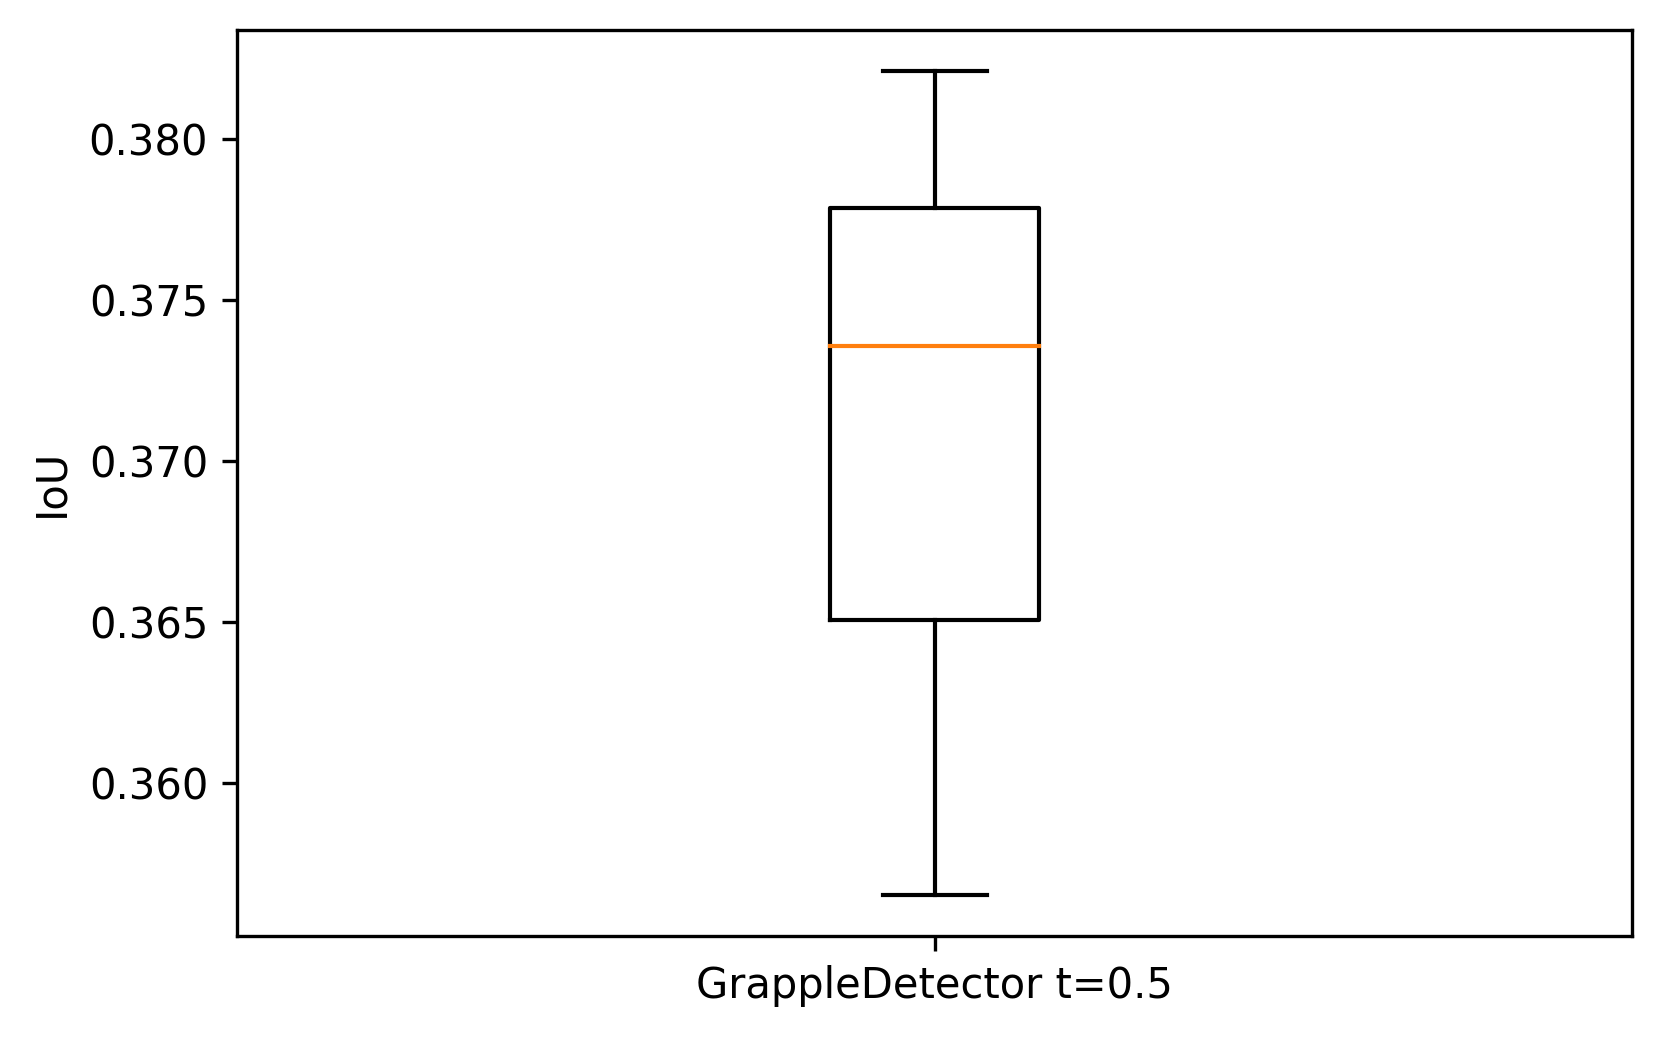
\includegraphics[width=1\textwidth,center]{bilder/Hauptteil/Autoencoder_Grappel_Detection/IoU_05_AE_Grapple.png}
    		\caption{Schwellenwert 0.5}
    		\label{img:BoxPlot_RegressionAufAutoencoder05}	
    	\end{subfigure}
    	\centering
    \begin{subfigure}[c]{0.29\textwidth}			
    	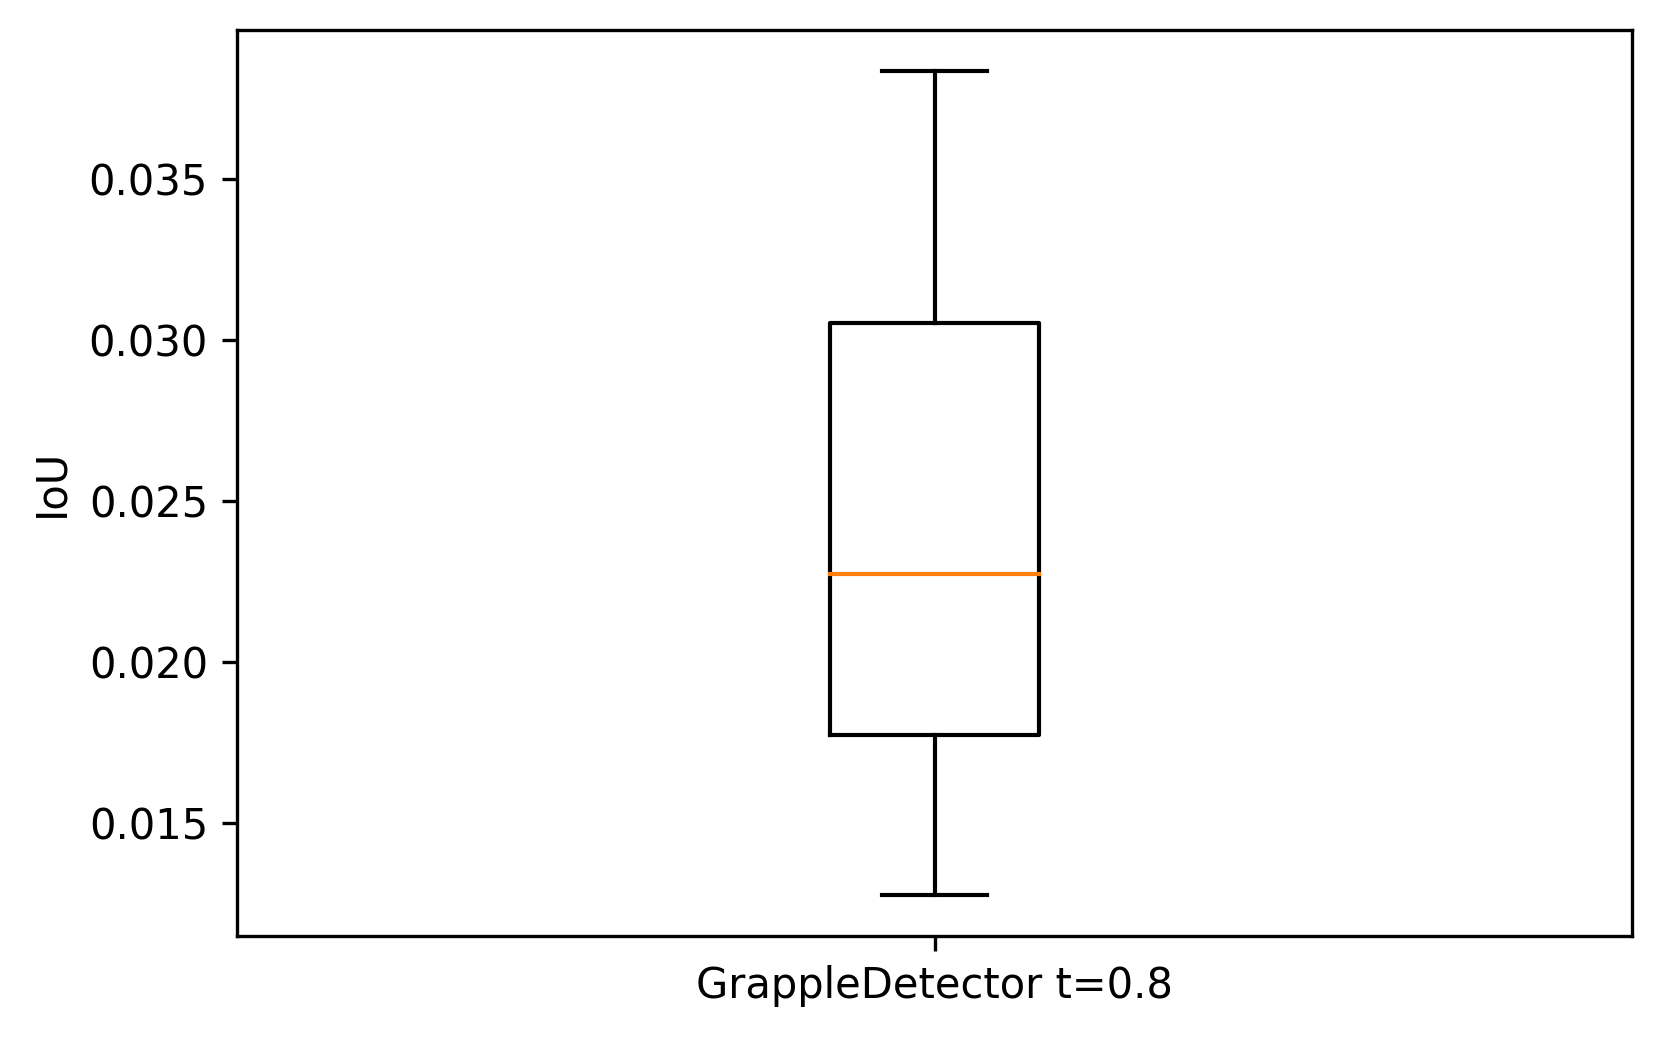
\includegraphics[width=1\textwidth,center]{bilder/Hauptteil/Autoencoder_Grappel_Detection/IoU_08_AE_Grapple.png}
    	\caption{Schwellenwert 0.8}
    	\label{img:BoxPlot_RegressionAufAutoencoder08}	
    \end{subfigure}
    	\begin{subfigure}[c]{0.29\textwidth}			
    		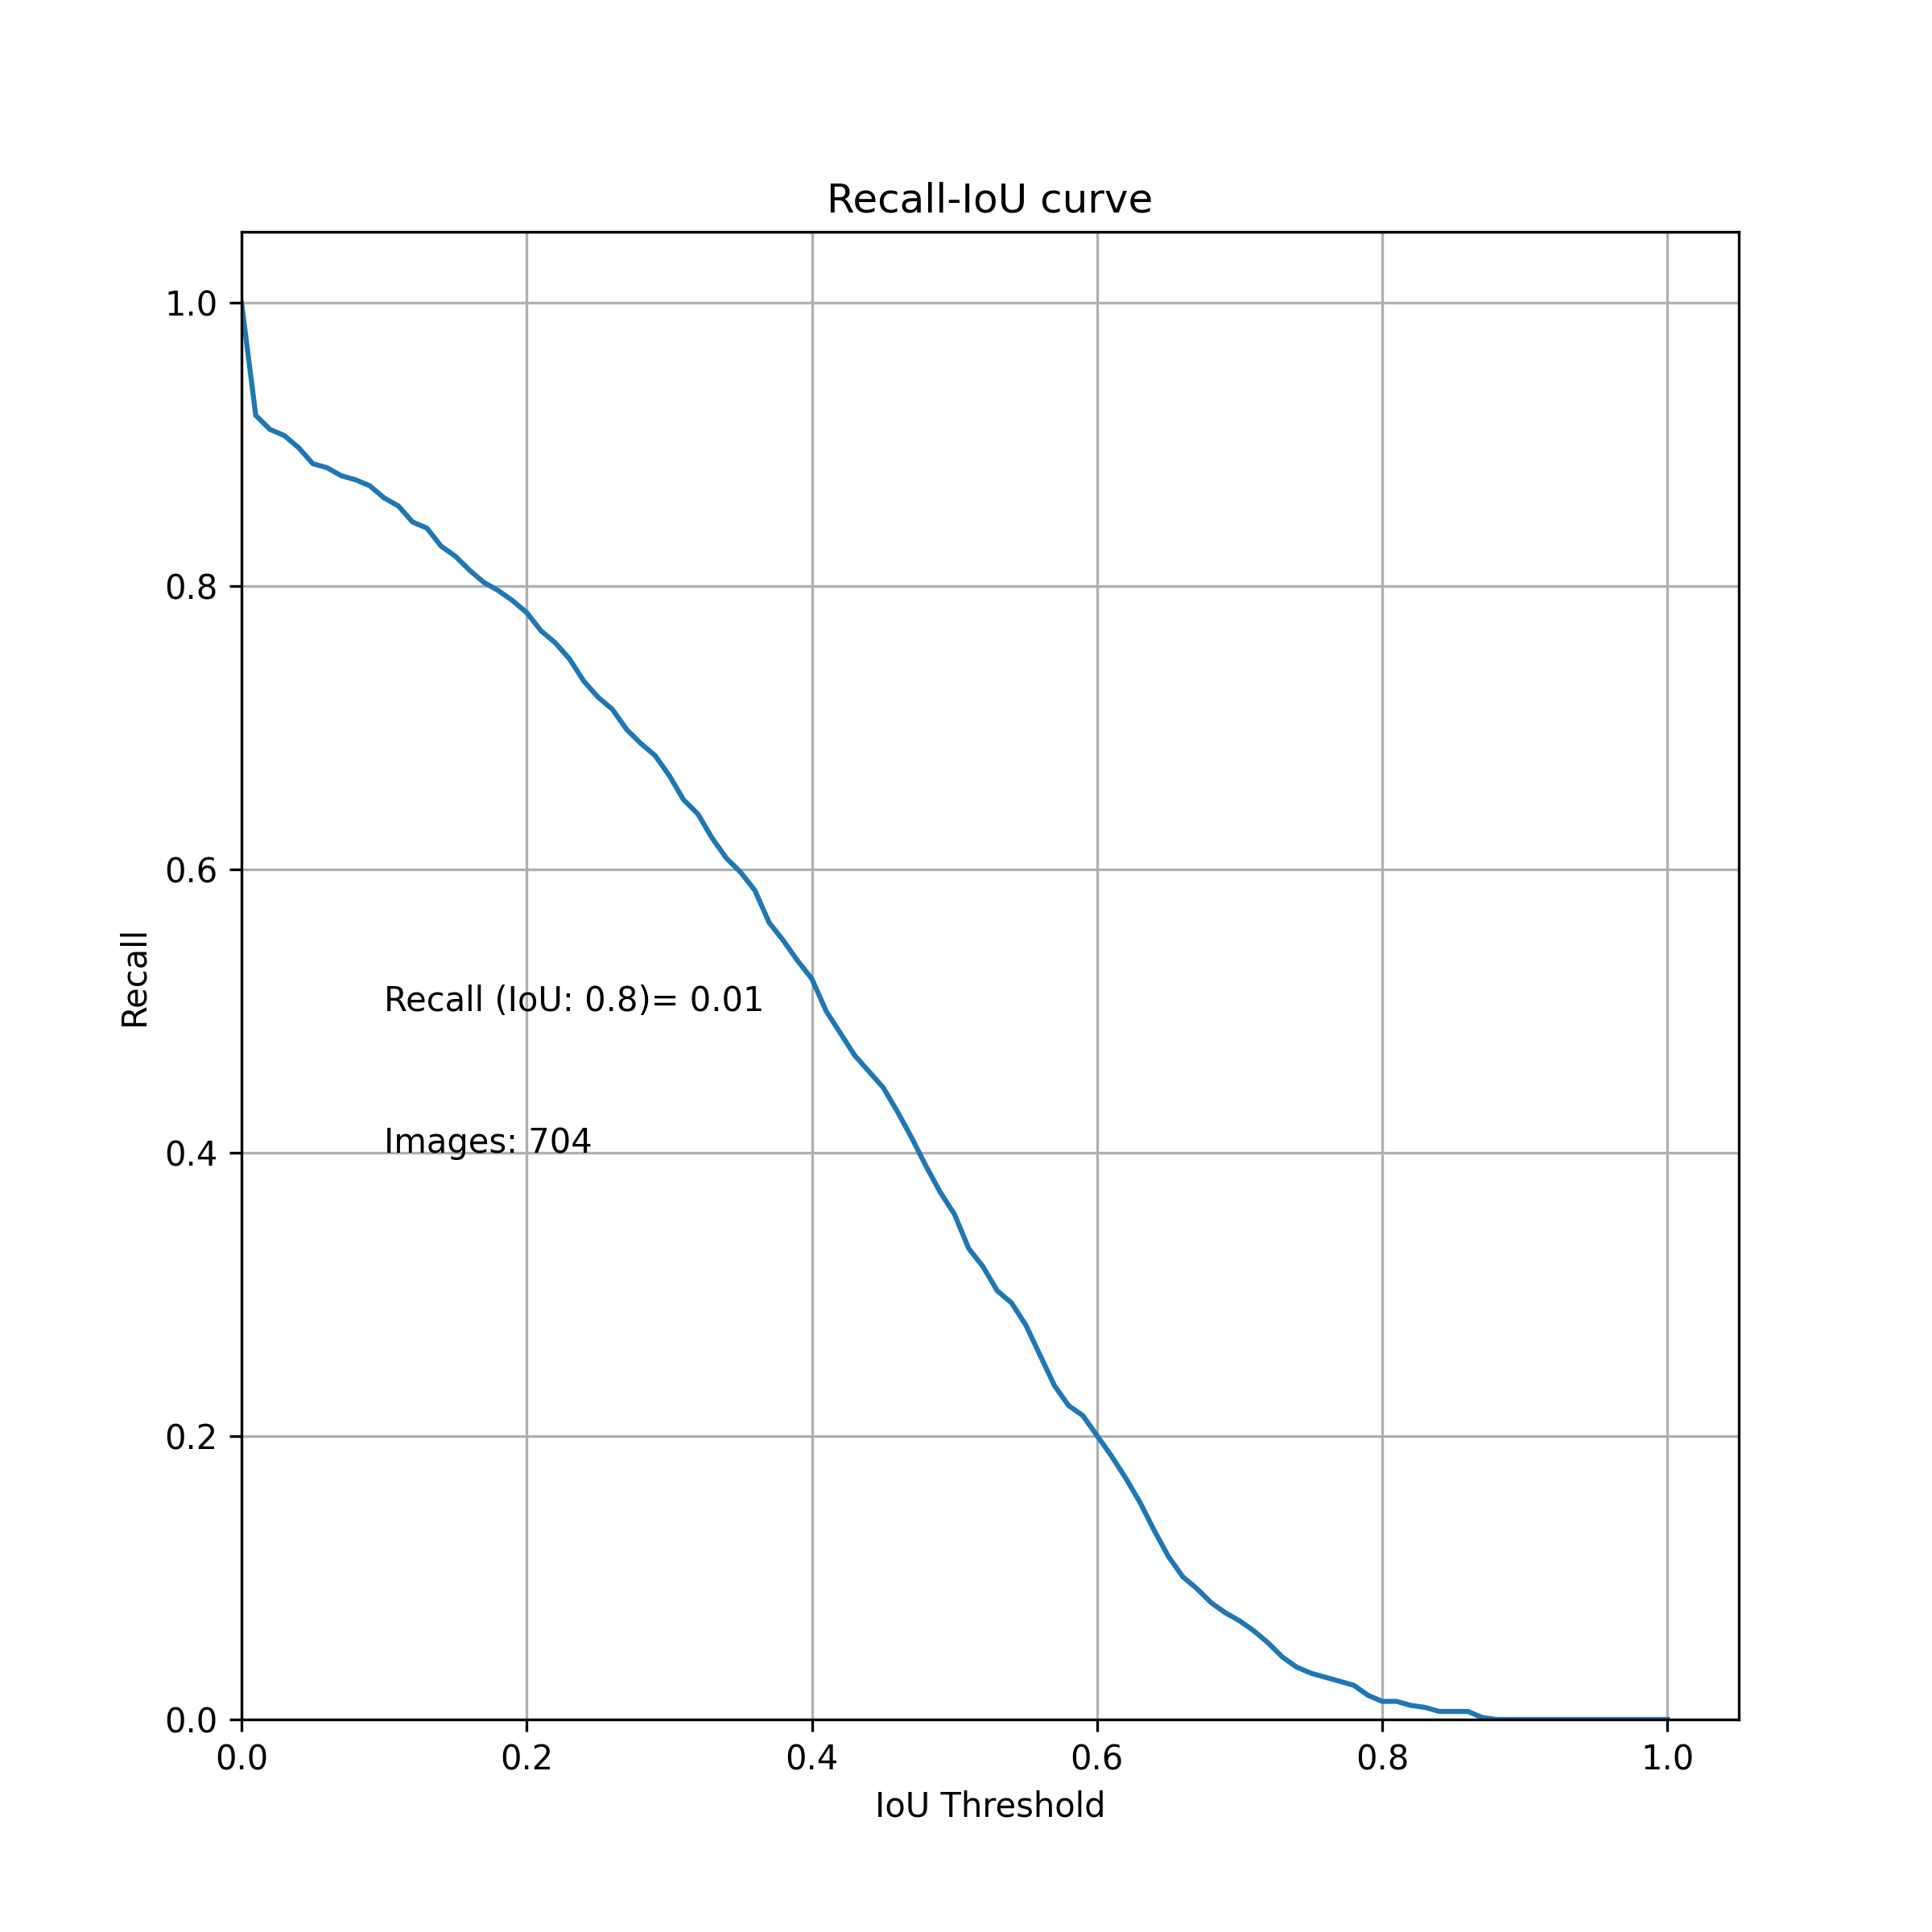
\includegraphics[width=1\textwidth, center]{bilder/Hauptteil/Autoencoder_Grappel_Detection/IoU.png}
    		\caption{Recall-IoU-Curve}
    		\label{img:RecalllIoUt_RegressionAufAutoencoder}	
    	\end{subfigure}
    	\caption{Ergebnis Regression auf Autoencoder}
        \label{img:ErgebnissRegressionAufAE}
    \end{figure}

	
	  \begin{figure}[h]
		\centering
		\begin{subfigure}[c]{0.49\textwidth}			
			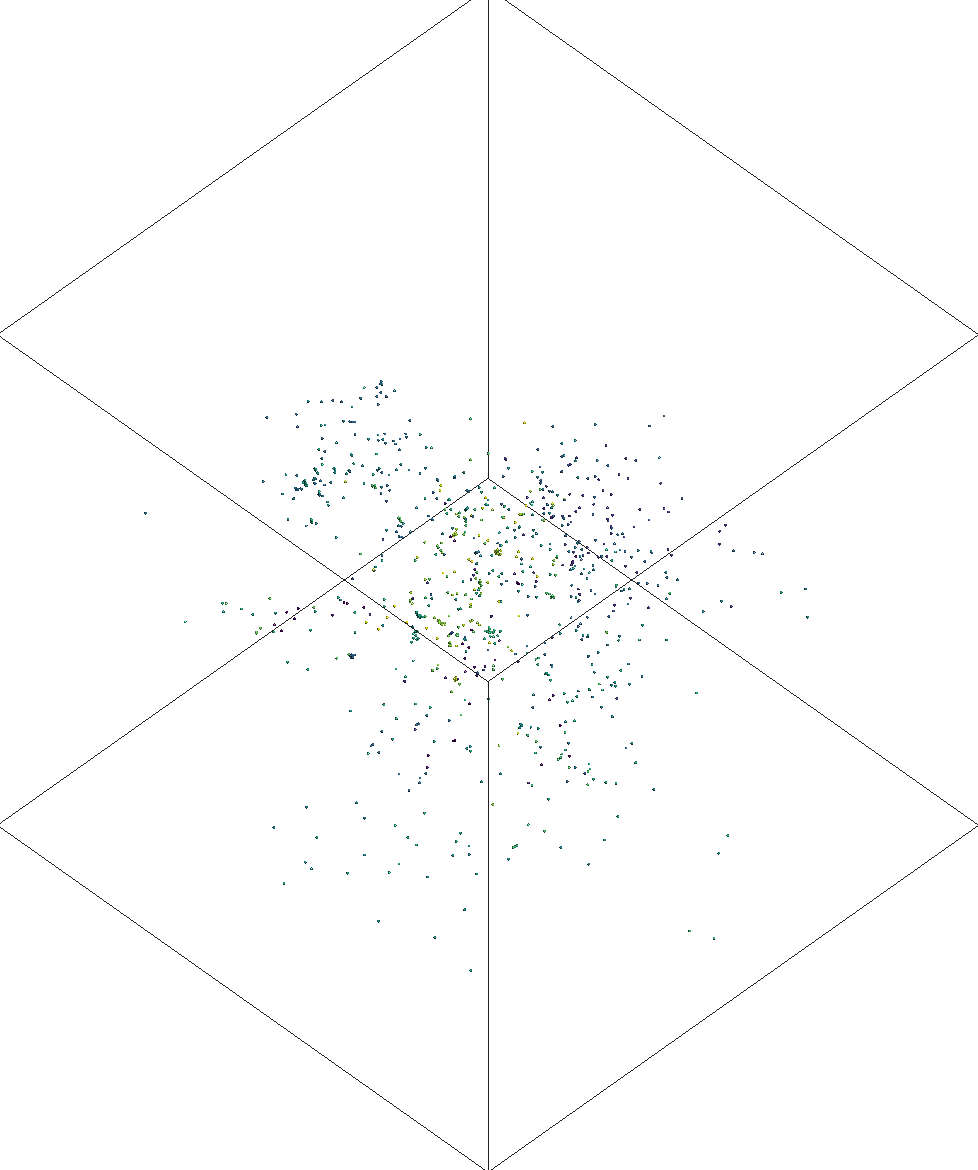
\includegraphics[width=1\textwidth,center]{bilder/Hauptteil/Autoencoder_Grappel_Detection/y_embKopie.png}
			\caption{Embedding mit y-Position des Greifers}
			\label{img:Emb_y_AE}	
		\end{subfigure}
		\begin{subfigure}[c]{0.49\textwidth}			
			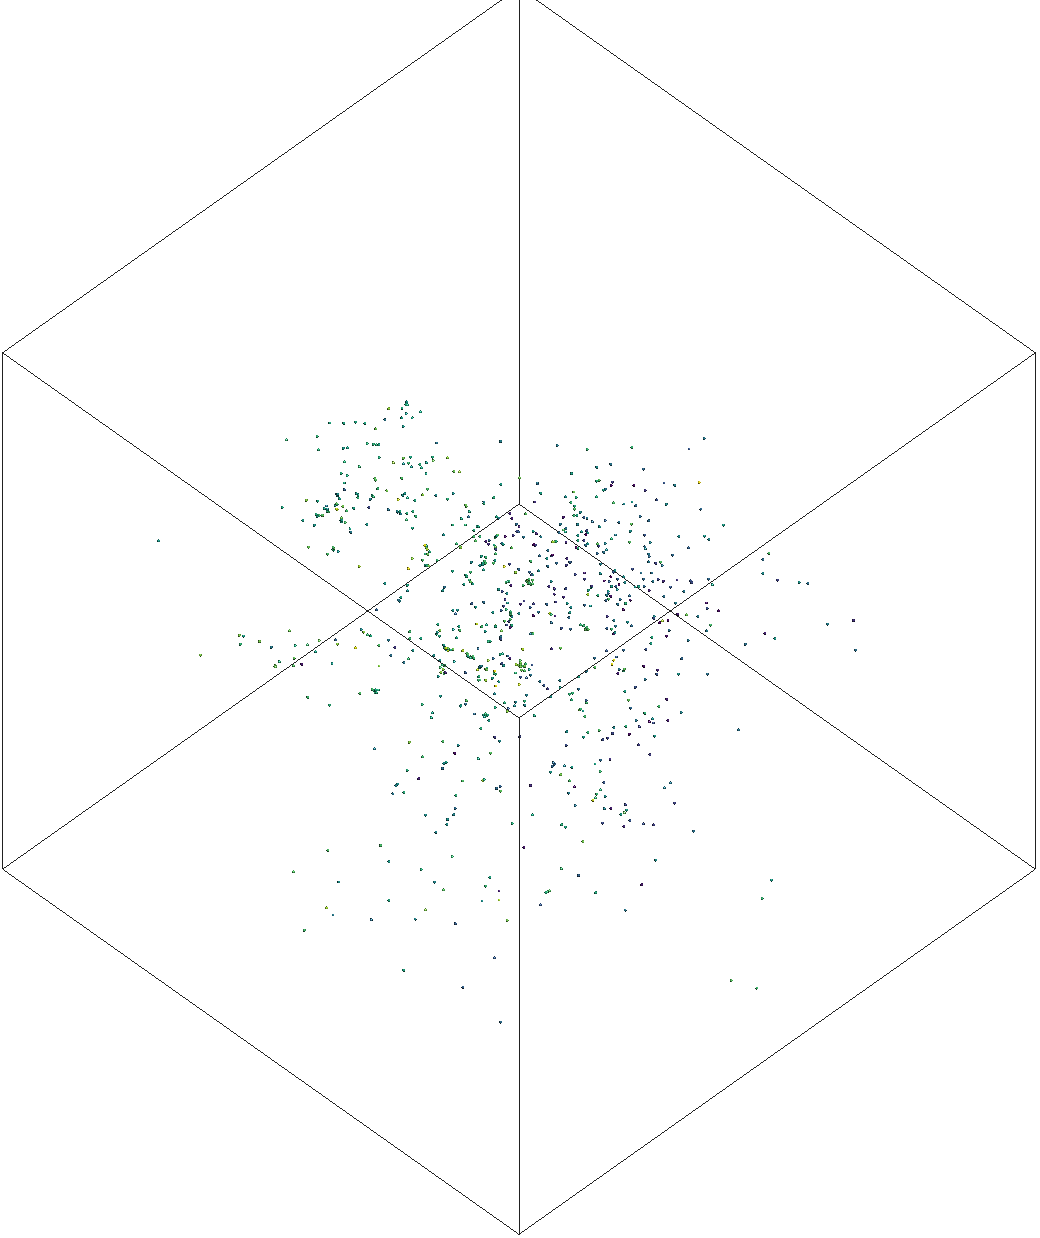
\includegraphics[width=1\textwidth, center]{bilder/Hauptteil/Autoencoder_Grappel_Detection/x_embKopie.png}
			\caption{Embedding mit x-Position des Greifers}
			\label{img:Emb_x_AE}	
		\end{subfigure}
		\caption{Embedding Autoencoder}
		\label{img:EmbeddingAE_V}
	\end{figure}
	
	\begin{figure}[h]
		\centering
		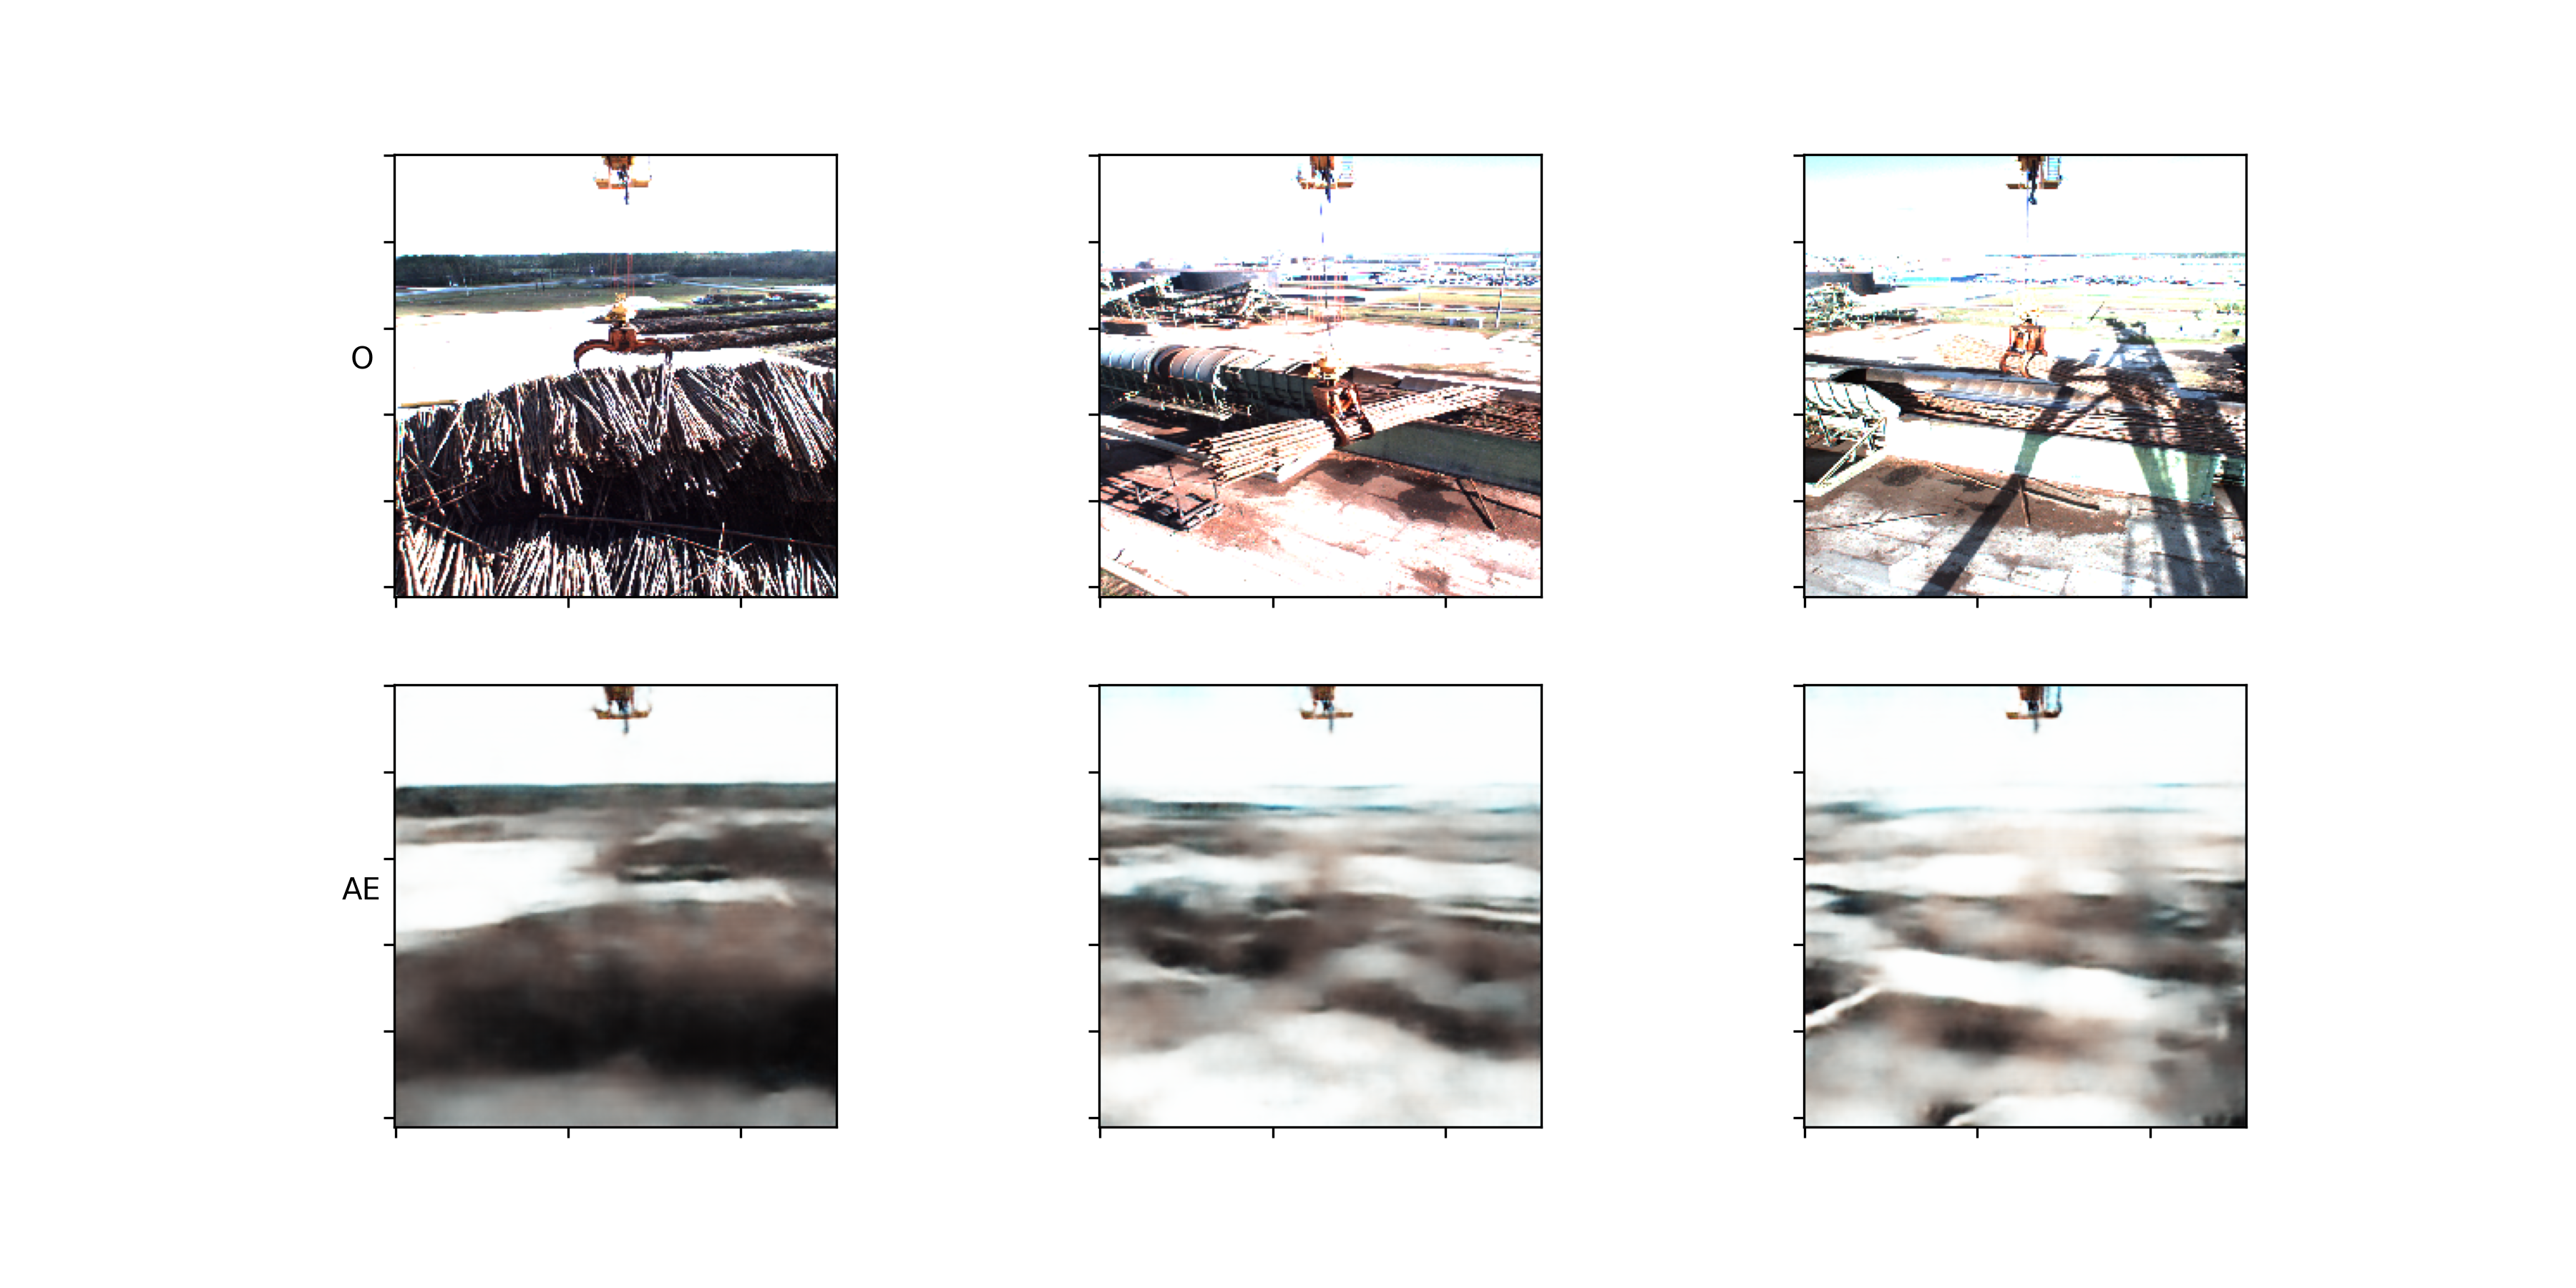
\includegraphics[width=1\textwidth, center]{bilder/Hauptteil/Autoencoder_Grappel_Detection/OriginalPicturesAndReconstruction.png}
		\caption{Rekonstruktion Autoencoder}
		\label{img:RekonstruktionAE}
	\end{figure}  
	
	
	
	\section{Aufgabenfokussierung und Greifererkennung}
	\label{sec:MultiTaskGreifererkennung}
	Im Ansatz \ref{sec:GreifererkennungAufAutoencoder} wurde die fehlende Fokussierung des Autoencoders auf den Greifer als Schwäche ausgemacht. Als neuer Ansatz wird untersucht, ob ein gleichzeitiges Lernen der Datenrepräsentation und das finden des Rahmens um den Greifer, den Autoencoder fokussiert und gleichzeitig gute Ergebnisse für die Regression gefunden werden können. Konkret wird ein \ac{mtl} \ac{simo} Ansatz untersucht.  
	
	\subsection{Werkzeug: TaskFocusingOnAutoencoder}
	\label{subsec:SecondCriterionAutoenocder}
	Zur Umsetzung des Ansatzes wurde ein Modul in Python erstellt. Da eine Aufgabe des Multi-Task-Ansatzes ein Autoencoder ist, wurde als Basis die Klasse ConvolutionalAutoencoder des Moduls autoencoder.py genutzt. Es wurde ein neues Modul erstellt, welches zusätzlich zu der Rekonstruktion des Autoencoders einen weiteren Ausgang bereitstellt. Der weitere Ausgang kann, wie jeder Ausgang für eine Binärklassifikation, für eine Multiklassifikation, für eine Regression oder jede andere beliebige Aufgabe genutzt werden. In Abbildung \ref{img:SchemaTFAE} ist der schematische Aufbau des Ansatzes abgebildet. Die Schichten des weiteren Kriteriums werden an die Code-Schicht des Autoencoders angehängt. Es können beliebig viele Schichten genutzt werden. Die Verlustfunktion des neuronalen Netzwerkes besteht aus der Summe der einzelnen Verlustfunktionen und einer Gewichtung. Sie lautet im Detail: 
	\begin{align}
	loss = weight1 * loss\_autoencoder + weight2 * loss\_task2
	\end{align}
	Die Gewichtung der Verlustfunktionen wird per Konstruktor-Argument übergeben. In Abbildung \ref{img:KlassendiagrammTFAE} ist das Klassendiagramm des TaskFocusingOnAutoencoder kurz TFAE dargestellt.
	\begin{figure}[h]
		\centering
		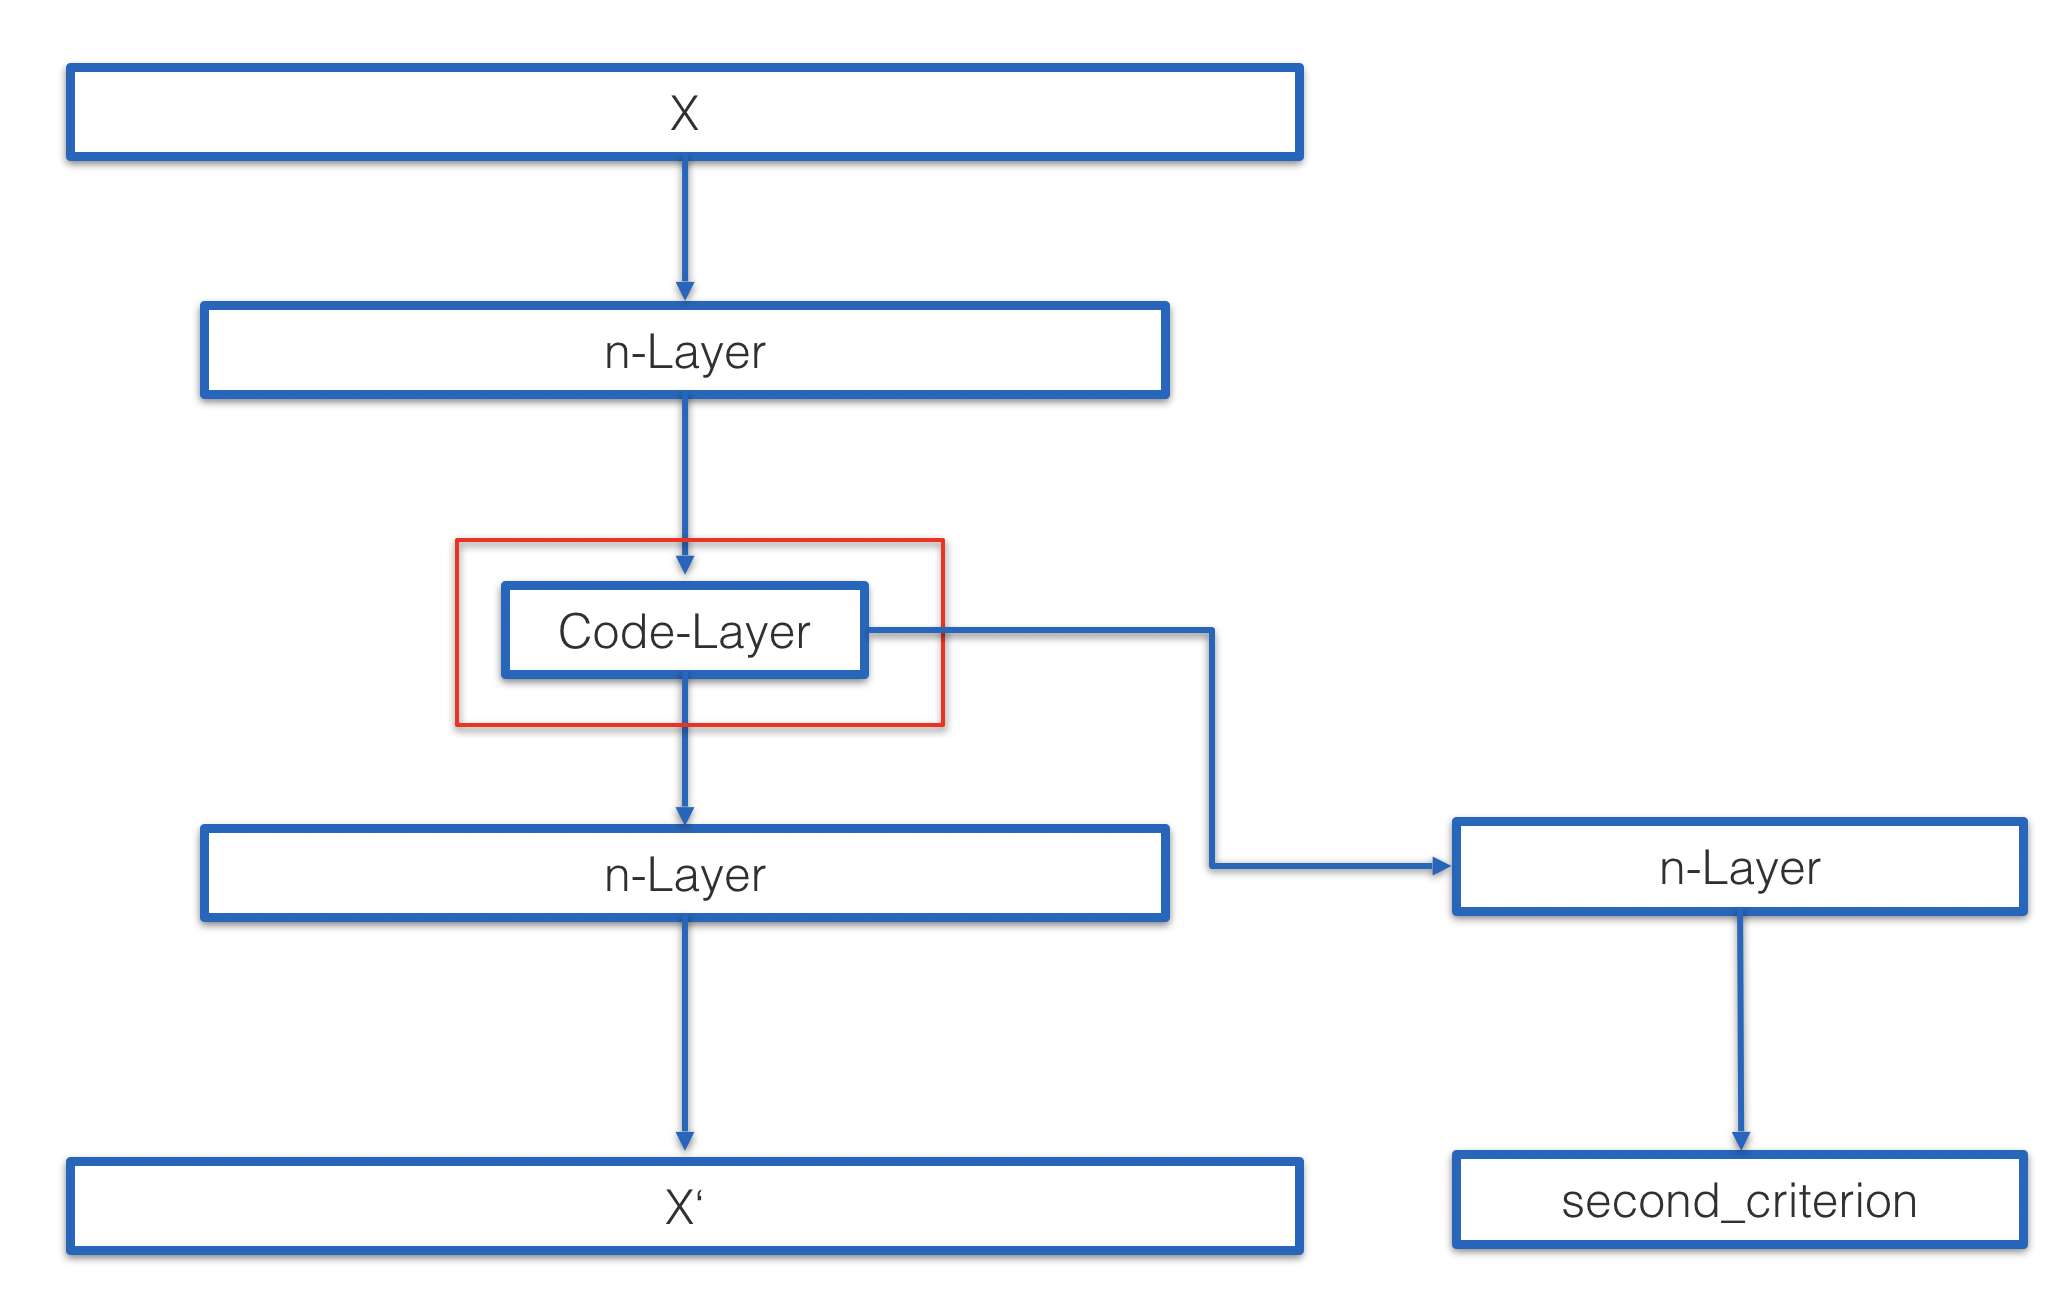
\includegraphics[width=0.7\textwidth, center]{bilder/Schema_Autoencoders/Schema_SCAE.png}
		\caption[Schema TaskFocusingOnAutoencoder]{Schema TaskFocusingOnAutoencoder}
		\label{img:SchemaTFAE}
	\end{figure}  
	\begin{figure}[h]
		\centering
		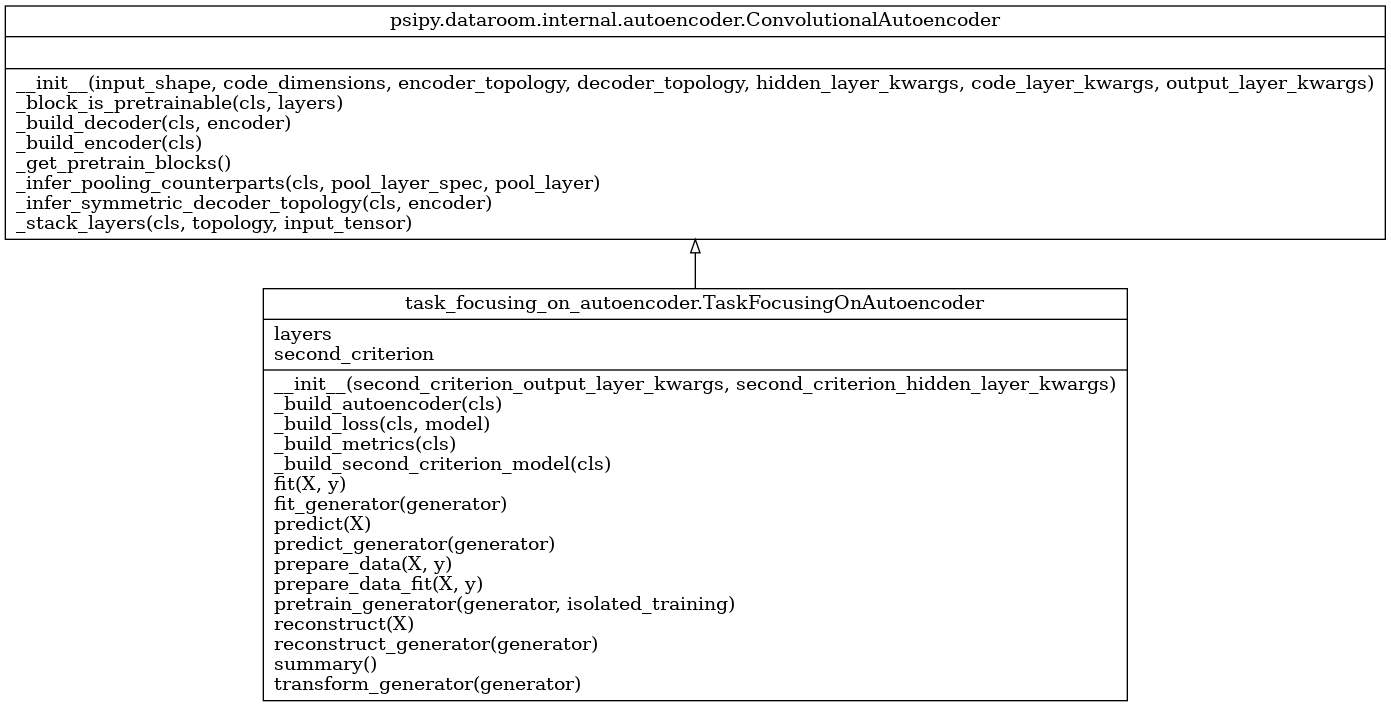
\includegraphics[width=0.7\textwidth, center]{bilder/Klassendiagramme/TFAE.png}
		\caption[Klassendiagramm TaskFocusingOnAutoencoder]{Klassendiagramm TaskFocusingOnAutoencoder}
		\label{img:KlassendiagrammTFAE}
	\end{figure}  
	Über den Konstruktor können alle Argumente, welche zum Erstellen des Models notwendig sind, per doppeltes Sternchen Wörterbuch Argument (**kwargs) an die Klasse übergeben werden. Diese Technik erlaubt es, eine mit Schlüsselwörtern versehene Argumentliste variabler Länge zu übergeben. Die Argumentlisten werden beinahe in allen Methoden zum Einsatz gebracht. Sie werden insbesondere genutzt, um Argumente an die zugehörigen Keras-Methoden zu übergeben. Die Namensgebung der Methode orientiert sich dabei an Keras. So wird z. B. in dem Methodenaufruf $fit(..)$ unter anderem auch die Keras-Methode $fit(..)$ aufgerufen. Um einen TFAE zu trainieren, ist es notwendig eine Instanz zu erzeugen, die Methode $pretrain(..)$ aufzurufen und ihn anschließend mit der Methode $fit(..)$ zu trainieren.
	In dem Methodenaufruf $pretrain(..)$ wird das Modell erstellt und schichtenweise vortrainiert. Das eigentliche Training erfolgt in der Methode $fit(..)$. Alternativ können auch die zugehörigen Generatorenklassen aufgerufen werden.    

	In Listing \ref{lst:BspErstellungConvolutionalSecondCriterionAutoenocder} ist beispielhaft dargestellt, wie ein TFAE erstellt wird. In den ersten 10 Zeilen wird die Architektur erstellt. Ab Zeile 12 wird eine Instanz eines TFAE mittels Argumentenliste erstellt. Zu beachten ist, dass hier keine Decoder-Architektur übergeben wird. Wenn keine Decoder-Architektur bereitgestellt wird, wird sie beim Erstellen des eigentlichen Modells aus der Encoder-Architektur abgeleitet.
	\begin{lstlisting}[language=python,caption=Beispiel Erstellung ConvolutionalSecondCriterionAutoenocder in Python, label=lst:BspErstellungConvolutionalSecondCriterionAutoenocder]
	encoder_topology = [("Conv2D", {"filters": 8, "kernel_size": (3, 3)}),
	("Conv2D", {"filters": 8, "kernel_size": (3, 3)}),
	('MaxPooling2D', {"pool_size": (2, 2)}),
	("Conv2D", {"filters": 16, "kernel_size": (3, 3)}),
	("MaxPooling2D", {"pool_size": (2, 2)}),
	("Conv2D", {"filters": 16, "kernel_size": (3, 3)}),
	("Flatten", {}),
	("Dense", {"units": 16})]

	second_criterion_topology = [("Dense", {"units": num_classes}) ]

	tfae = TaskFocusingOnAutoencoder(
	input_shape=(28, 28, 1),	
	code_dimensions=3, 
	encoder_topology=encoder_topology,
	second_criterion_topology=second_criterion_topology,
	hidden_layer_kwargs = {'activation': 'relu'},
	output_layer_kwargs = {'activation': 'sigmoid'},
	second_criterion_hidden_layer_kwargs = {'activation': 'relu'},
	second_criterion_output_layer_kwargs = {'activation': 'softmax'},
	second_criterion_loss = 'categorical_crossentropy',
	loss_weights=[8., 1.],
	second_criterion_metrics = {'second_criterion':'accuracy'},
	code_layer_kwargs=dict())
	\end{lstlisting}
	Listing  \ref{lst:BspPretrainConvolutionalSecondCriterionAutoenocder}  zeigt den Aufruf der Methode Pretrain. Der Aufruf führt zu einem Schichtenweise-Trainieren des Netzwerkes mit den Daten x\_train bei 20 Epochen und einer Stapelgröße von 64. 
	\begin{lstlisting}[language=python,caption=Beispielaufruf Pretrain  in Python, label=lst:BspPretrainConvolutionalSecondCriterionAutoenocder]
	tfae.pretrain(x_train,epochs = 20, batch_size = 64)
	\end{lstlisting}

	Der Methodenaufruf $fit(..)$ funktioniert wie der $fit(..)$-Aufruf in Keras. In Zeile drei des Listing  \ref{lst:BspPretrainConvolutionalSecondCriterionAutoenocder}  ist zu erkennen, dass die Zielgrößen der verschiedenen Ausgänge einfach als Python-Wörterbuch übergeben werden können.
	\begin{lstlisting}[language=python,caption=Beispielaufruf Fit  in Python, label=lst:BspFitConvolutionalSecondCriterionAutoenocder]
	history = tfae.fit(
		x_train,
		{"decoder": x_train, "second_criterion": y_train}, 
		epochs=200,
		batch_size = 64,
		validation_data=(x_test,{"decoder": x_test, "second_criterion": y_test})
	)
	\end{lstlisting}

	\subsection{Experiment}
	Mit dem \ac{tfae} wird für die Aufgabe 'Greifererkennung' im Median für den Schwellenwert 0.5 eine Leistung von 98.66\% erreichr, für den Schwellenwert von 0.8 eine Leistung von 66.62\%. In Abbildung \ref{img:ErgebnisRegressionMT} sind die Ergebnisse im Detail dargestellt. In Anhang \ref{appendix:MutliTaskGreifererkennung}	ist eine detailierte Einzelaufstellung der Ergebnisse zu finden. Diese Leistung ist deutlich besser, als die erzielte Leistung mit dem Ansatz 'Greifererkennung auf Repräsentation' \ref{sec:GreifererkennungAufAutoencoder}. Bei Betrachtung der Repräsentation in Abbildung \ref{img:EmbeddingMT} ist eine deutliche Anpassung an den Greifer zu erkennen. Sowohl die Farbkodierung für die y-Position als auch die x-Position des Greifers im Bild ist sehr deutlich zu erkennen. Zusätlich lässt sich eine Trennung der einzelnen Datenpunkte in das Merkaml Greifer ist offen oder Geschlossen erkennen. Es zieht sich eine sichtbare Trennung der Datenpunkte durch die Einbettung. Bei Betrachtung der Rekosntruktionen, insbesondere im direkten Vergleich zu den Rekonstruktionen des Autoencoders zeigt sich eine stärkere Ausprägung des Merkmales Greifer. In Abbildung \ref{img:RekonstruktionMTAE} sind drei Bilder mit ihren jeweiligen Rekosntruktionen dargestellt. Im Anhang \ref{appendix:MutliTaskGreifererkennung} ist eine größere Auswahl an Rekonstruktionen dargestellt.  
	
	Die Ergebnisse der sieben Versuche weißen insbesondere bei größeren Schwellenwerten eine starke Schwankung auf. In Abbildung \ref{img:Emb_MT_Vorhersage} sind in der Einbettung die Fehlvorhersagen lila eingefärbt. Die meisten Fehler sind bei geschlossenem Greifer entstanden. Werden die Einbettungen aller Versuche (\ref{appendix:MutliTaskGreifererkennung}) betrachtet, fällt auf, dass die x-Position des Greifers im Bild die herausfordernde Größe ist. Durch die zufällige Initalisierung der Gewichte kann in dem bestehdnen Setting nicht immer die beste Lösung gefunden werden. Die Robustheit der Lösung bei nidriegeren (bis circa 0.5) Schwellenwerten erlauben es aber dennoch die Lösung für weitere Versuche einzusetzen.
	    \begin{figure}[h]
		\centering
		\begin{subfigure}[c]{0.32\textwidth}			
			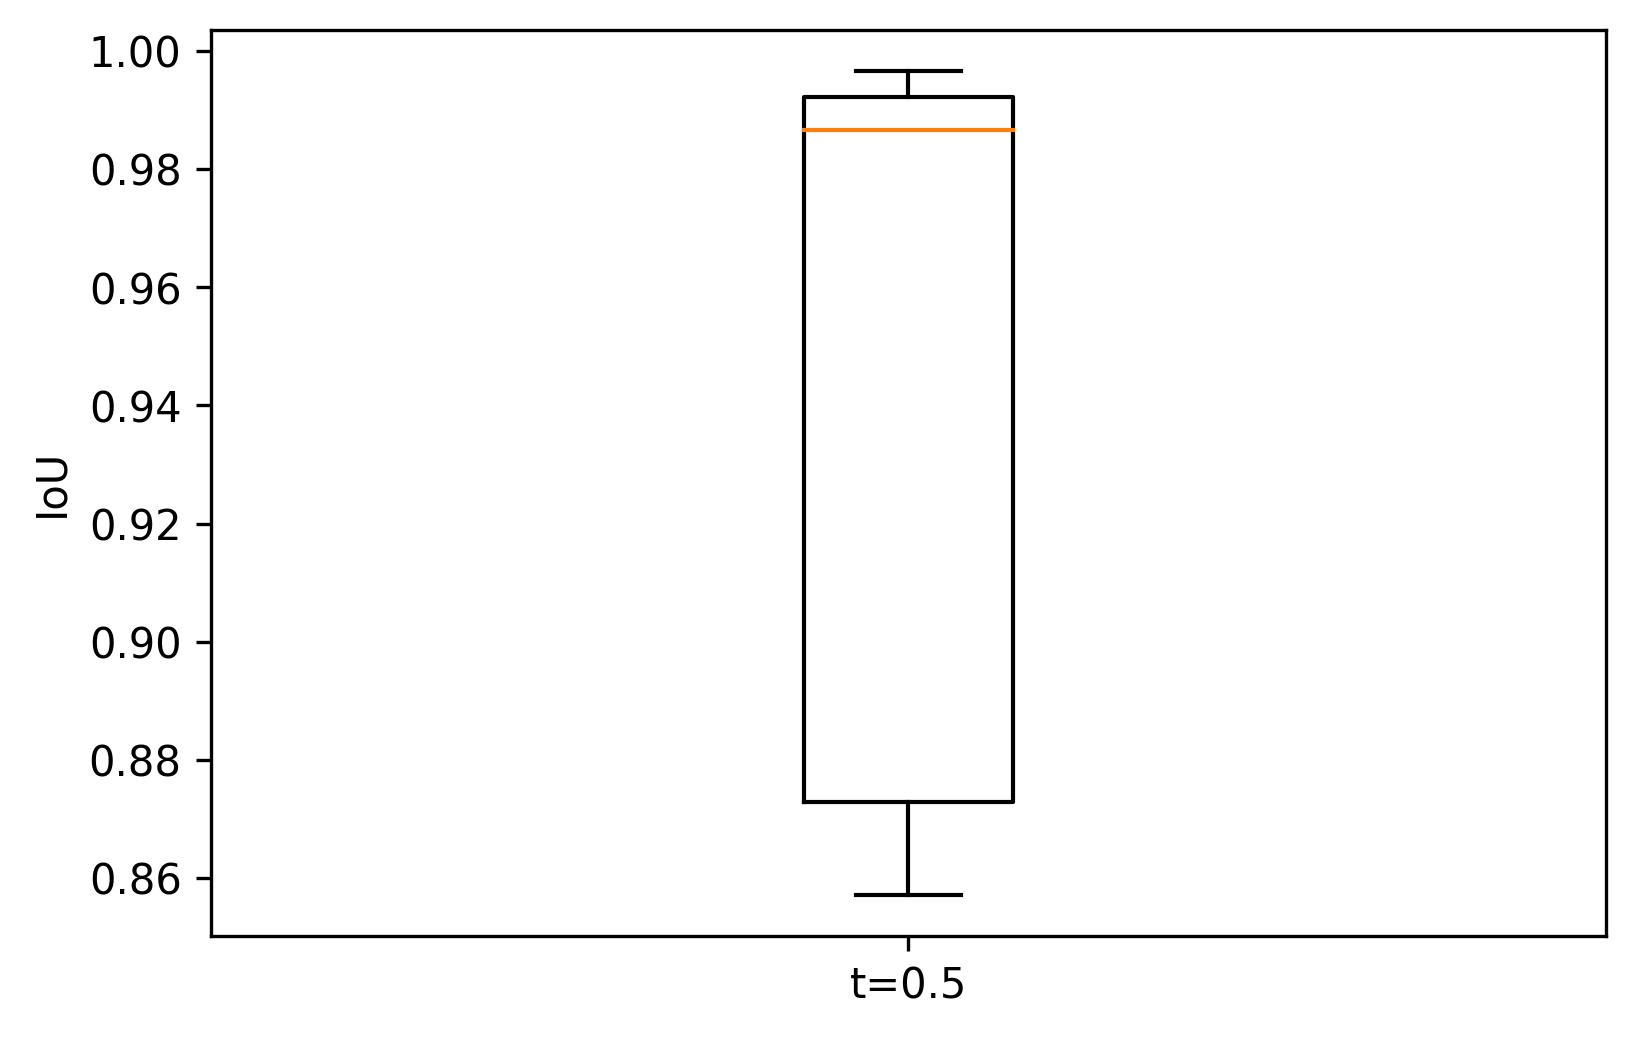
\includegraphics[width=1\textwidth,center]{bilder/Hauptteil/MT_Grapple/IoU_05_MT_Grapple.png}
			\caption{Schwellenwert 0.5}
			\label{img:BoxPlot_05_MT-Ansatz}	
		\end{subfigure}
		\centering
		\begin{subfigure}[c]{0.32\textwidth}			
			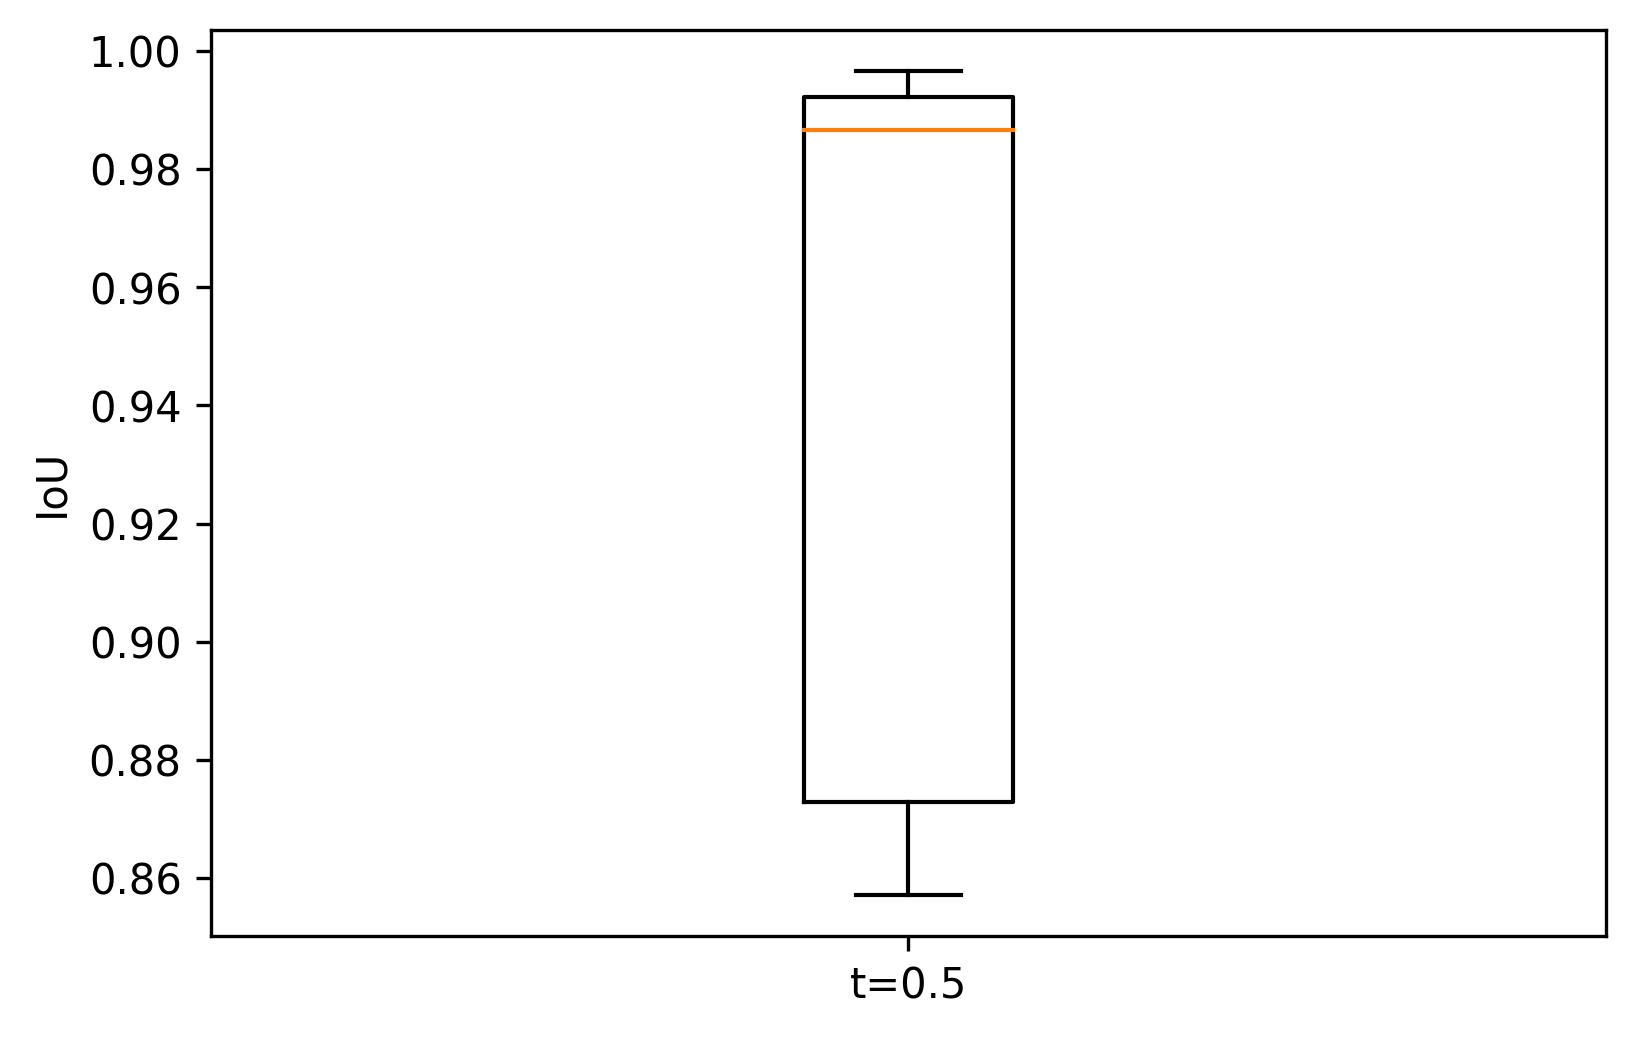
\includegraphics[width=1\textwidth,center]{bilder/Hauptteil/MT_Grapple/IoU_08_MT_Grapple.png}
			\caption{Schwellenwert 0.8}
			\label{img:BoxPlot_08_MT-Ansatz}	
		\end{subfigure}
		\begin{subfigure}[c]{0.32\textwidth}			
			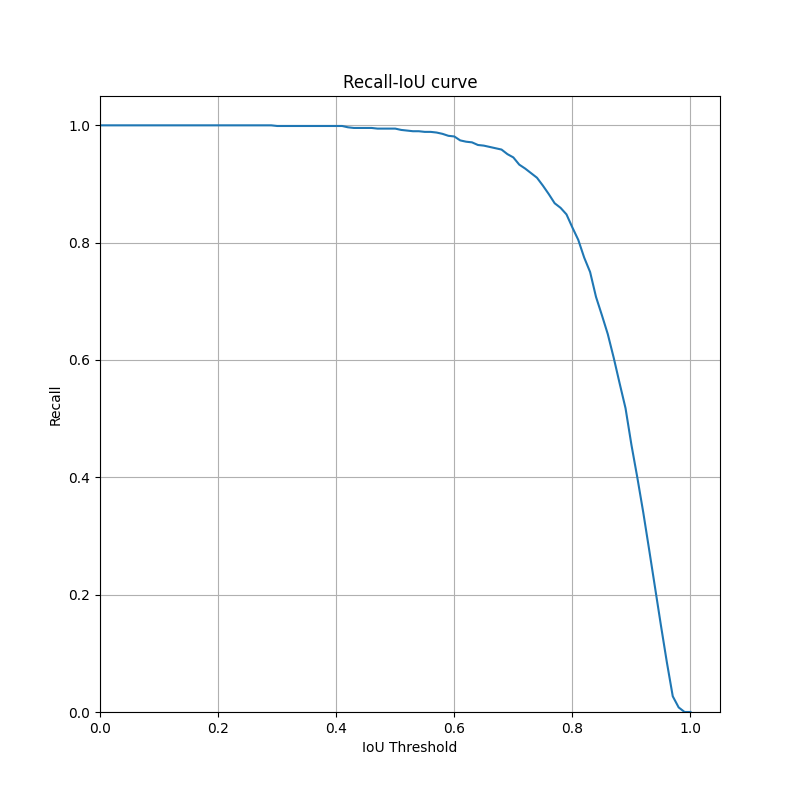
\includegraphics[width=1\textwidth, center]{bilder/Hauptteil/MT_Grapple/Recall_IoU.png}
			\caption{Recall-IoU-Curve}
			\label{img:RecalllIoUt_MT}	
		\end{subfigure}
		\caption{Ergebnis MT-Greifererkennung}
		\label{img:ErgebnisRegressionMT}
	\end{figure}

	
	\begin{figure}[h]
		\centering
		\begin{subfigure}[c]{0.49\textwidth}			
			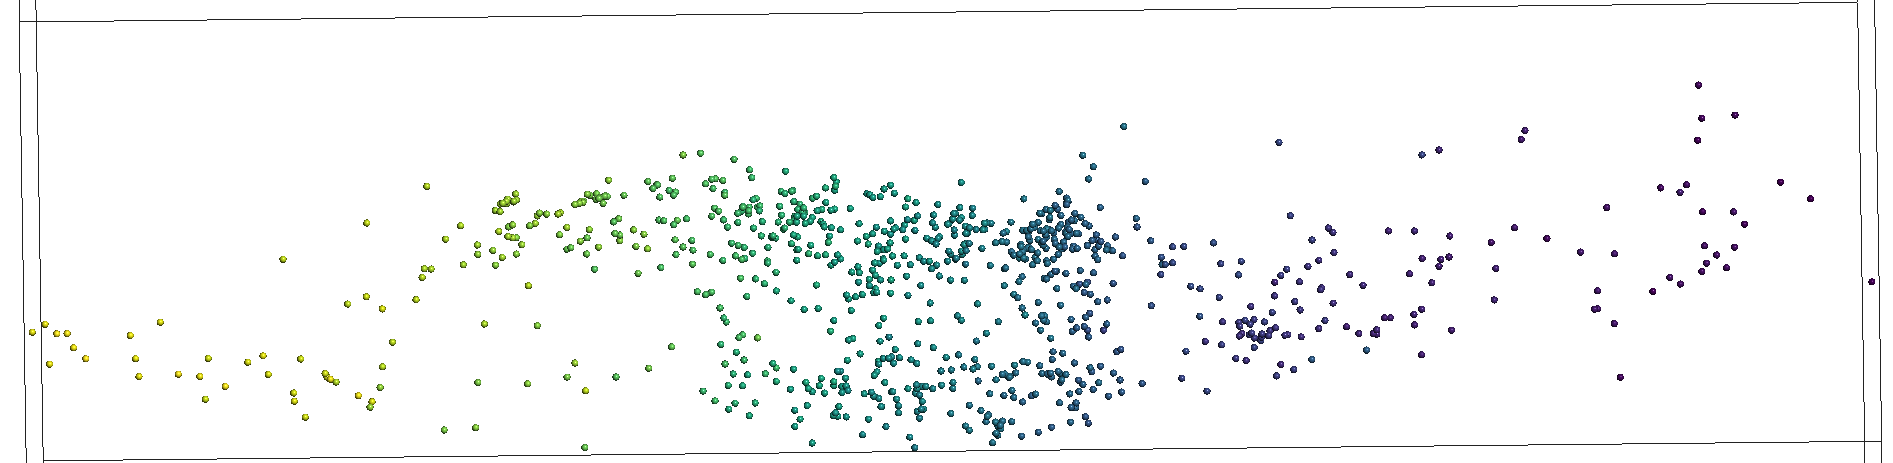
\includegraphics[width=1\textwidth,center]{bilder/Hauptteil/MT_Grapple/emb_y.png}
			\caption{Embedding mit y-Position des Greifers}
			\label{img:Emb_y_MT}	
		\end{subfigure}
		\begin{subfigure}[c]{0.49\textwidth}			
			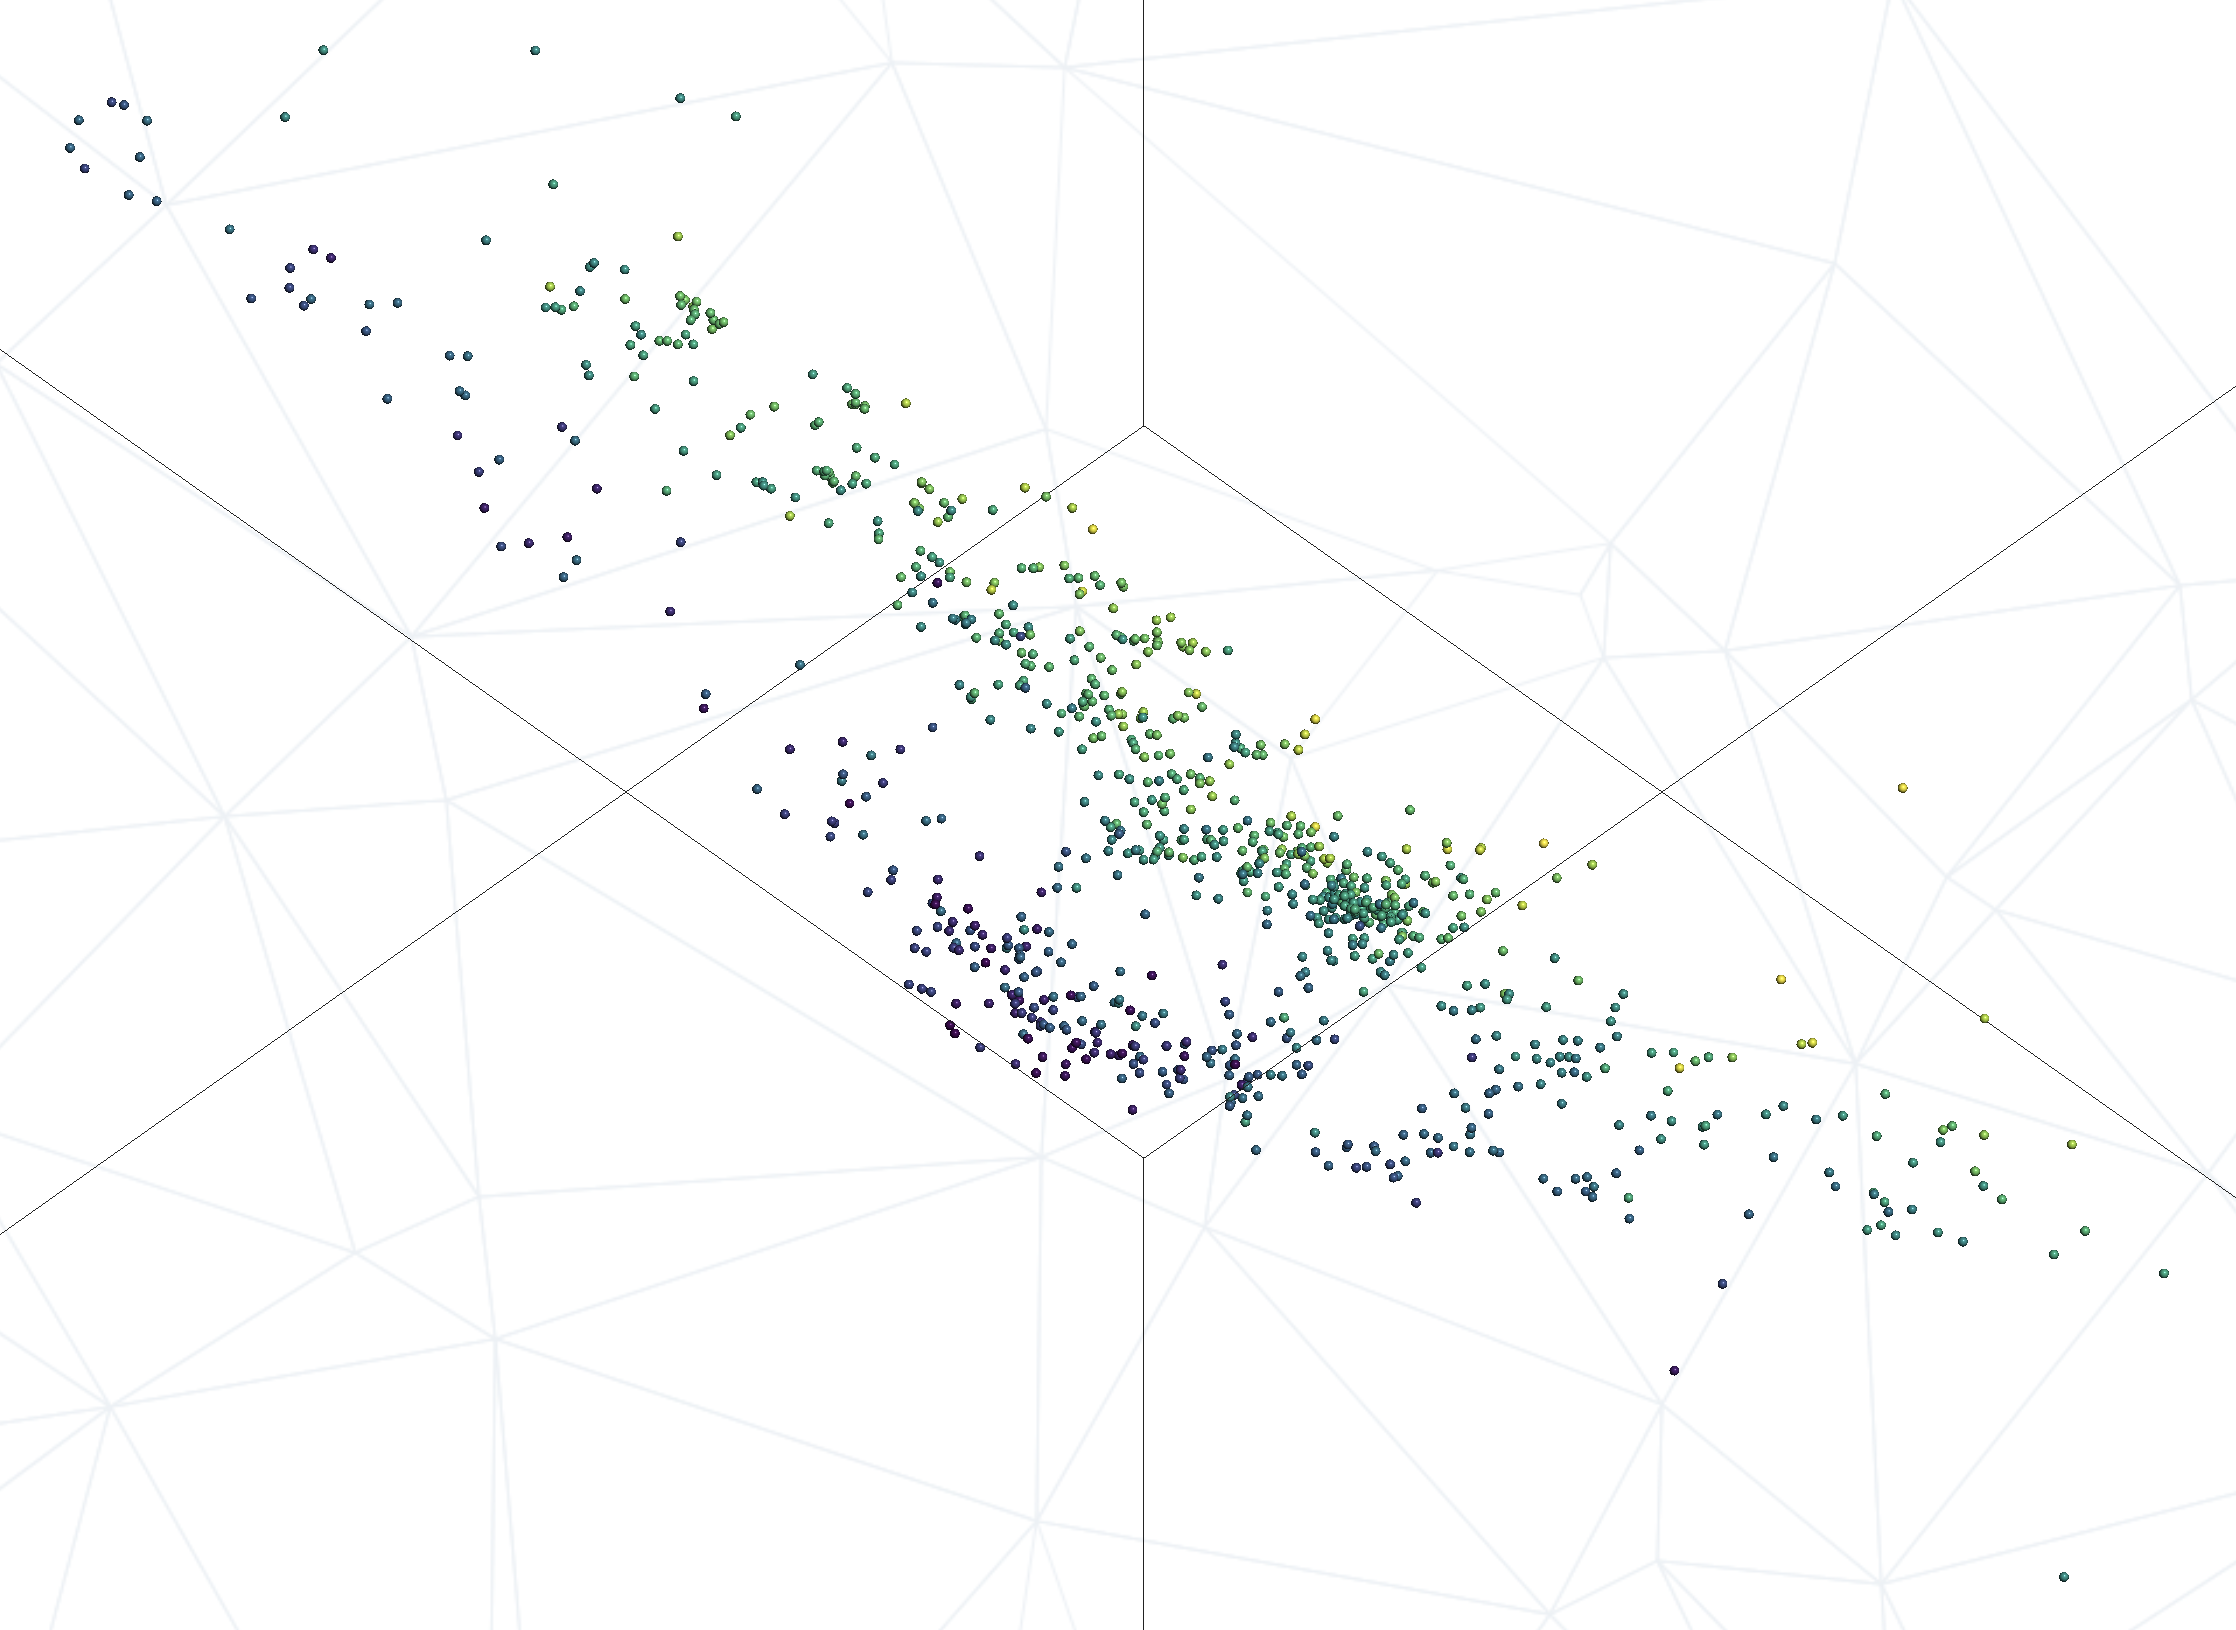
\includegraphics[width=1\textwidth, center]{bilder/Hauptteil/MT_Grapple/emb_x.png}
			\caption{Einbettung mit x-Position des Greifers}
			\label{img:Emb_x_MT}	
		\end{subfigure}
		\begin{subfigure}[c]{0.6\textwidth}			
		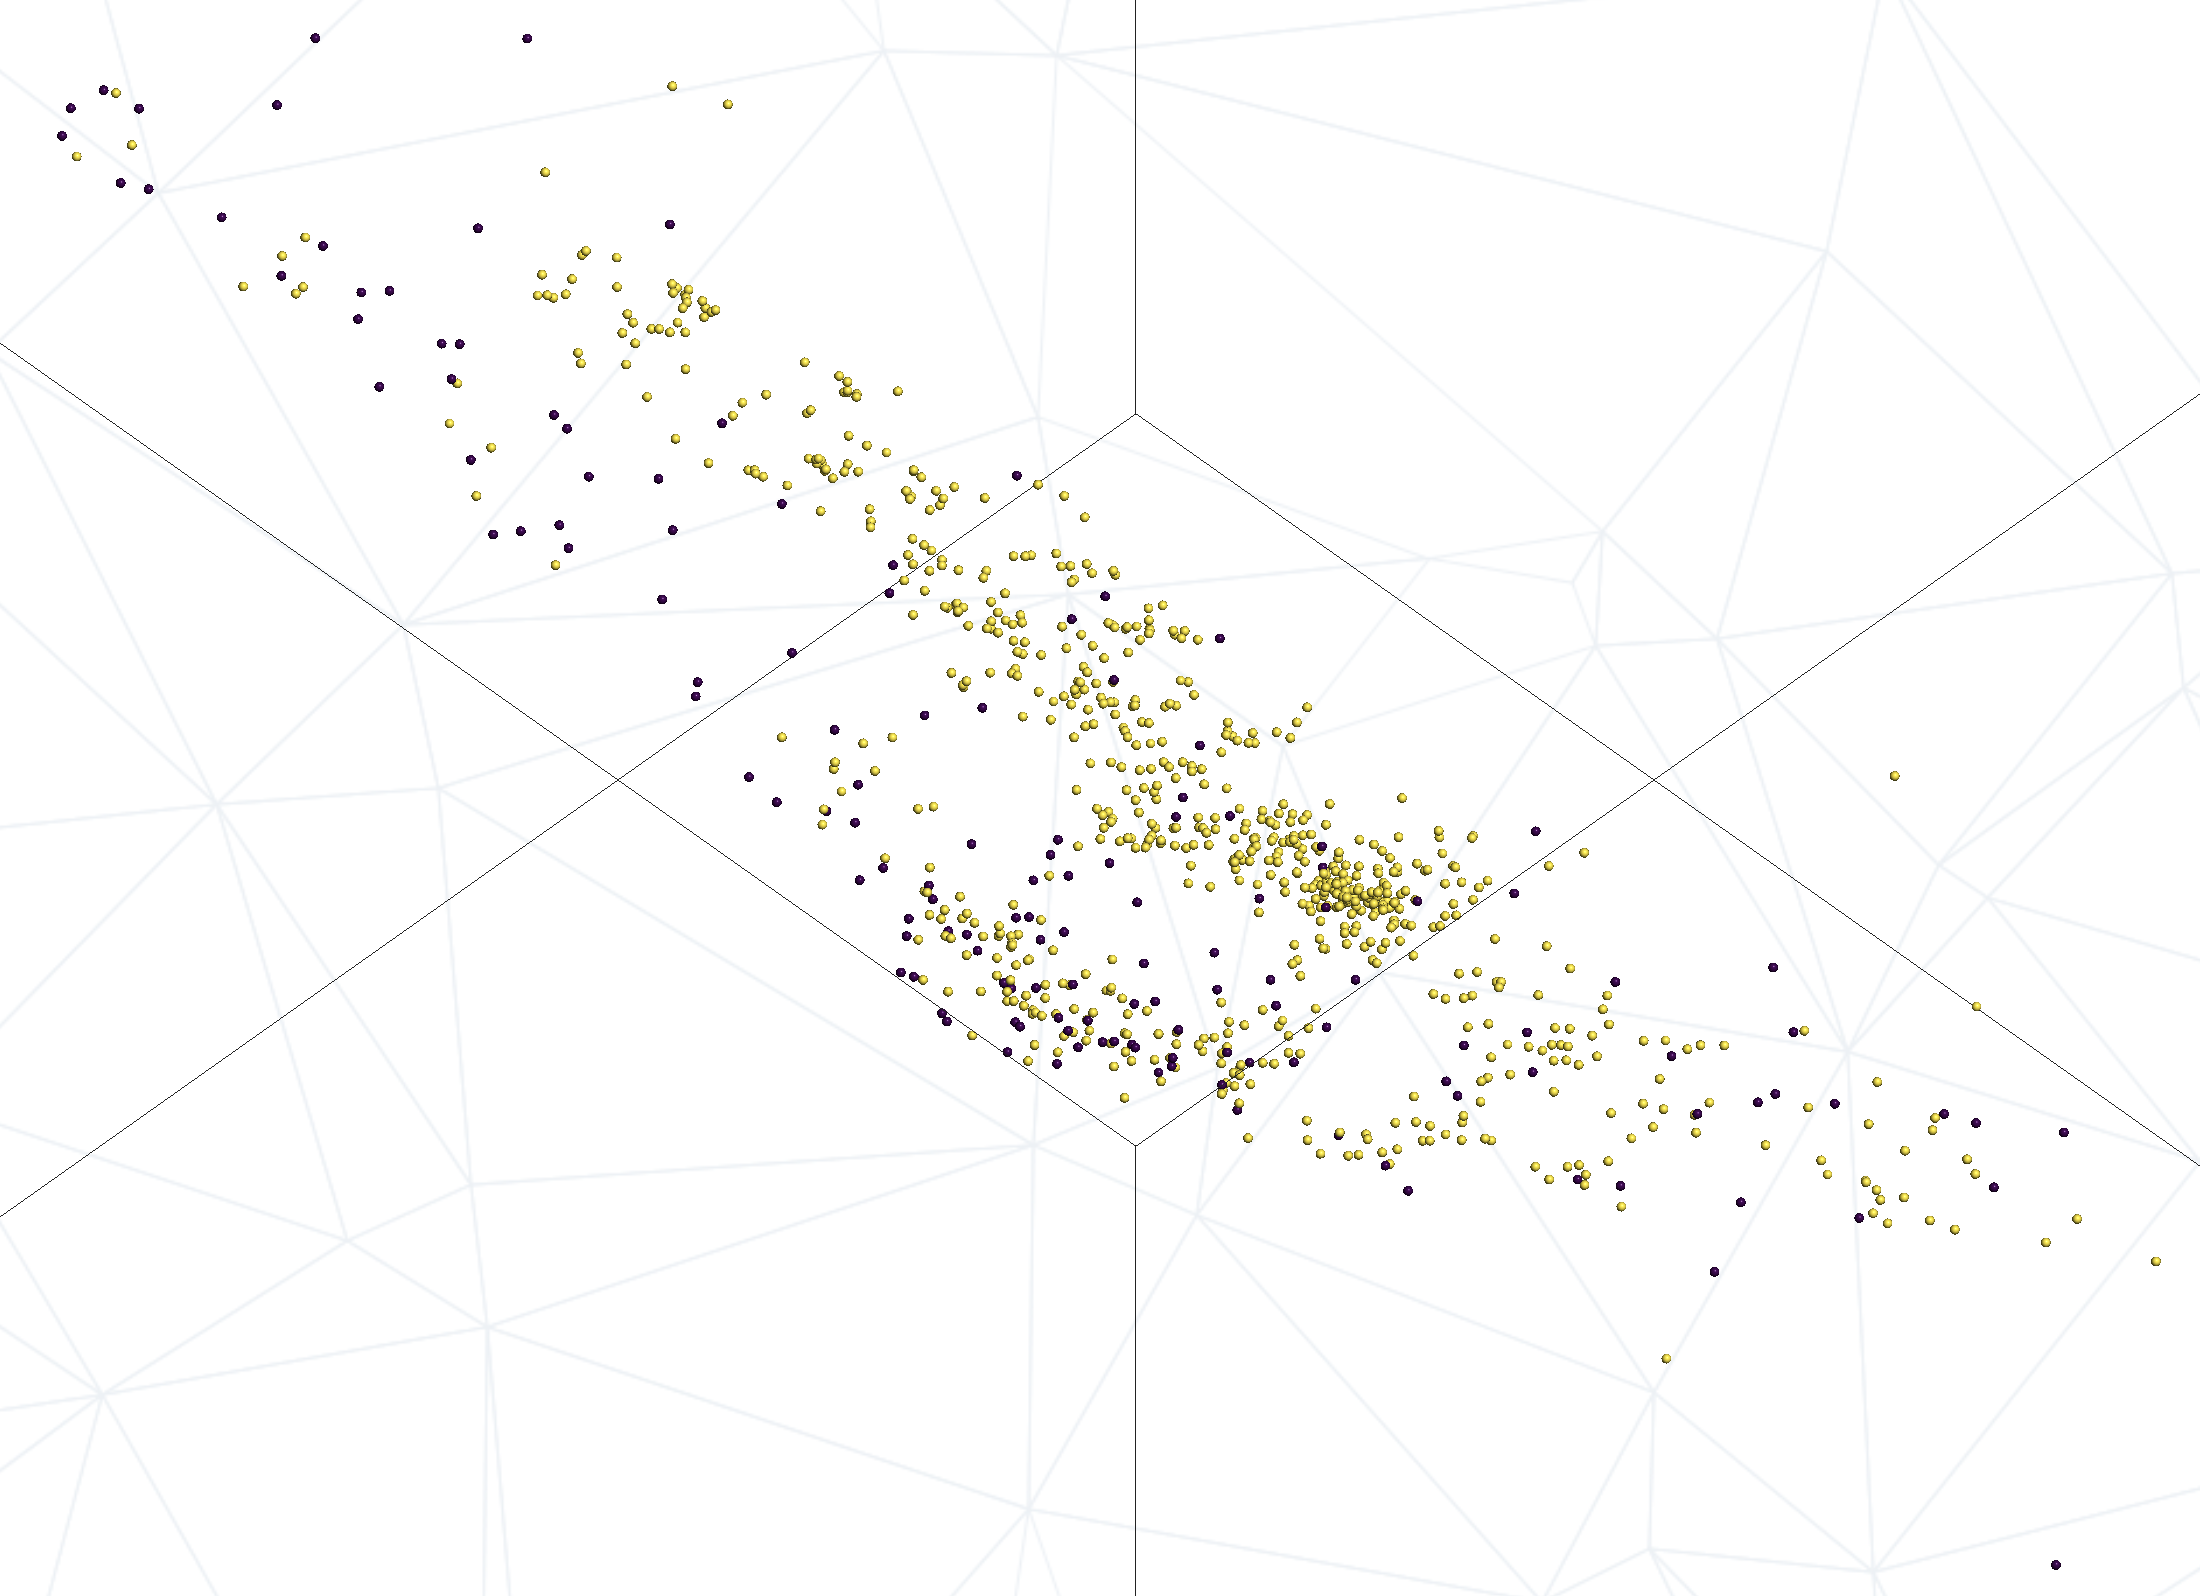
\includegraphics[width=1\textwidth, center]{bilder/Hauptteil/MT_Grapple/emb_res.png}
		\caption{Einbettung mit Vorhersage}
		\label{img:Emb_MT_Vorhersage}	
	\end{subfigure}
		\caption{Einbettung MT}
		\label{img:EmbeddingMT}
	\end{figure}
	
	\begin{figure}[h]
		\centering
		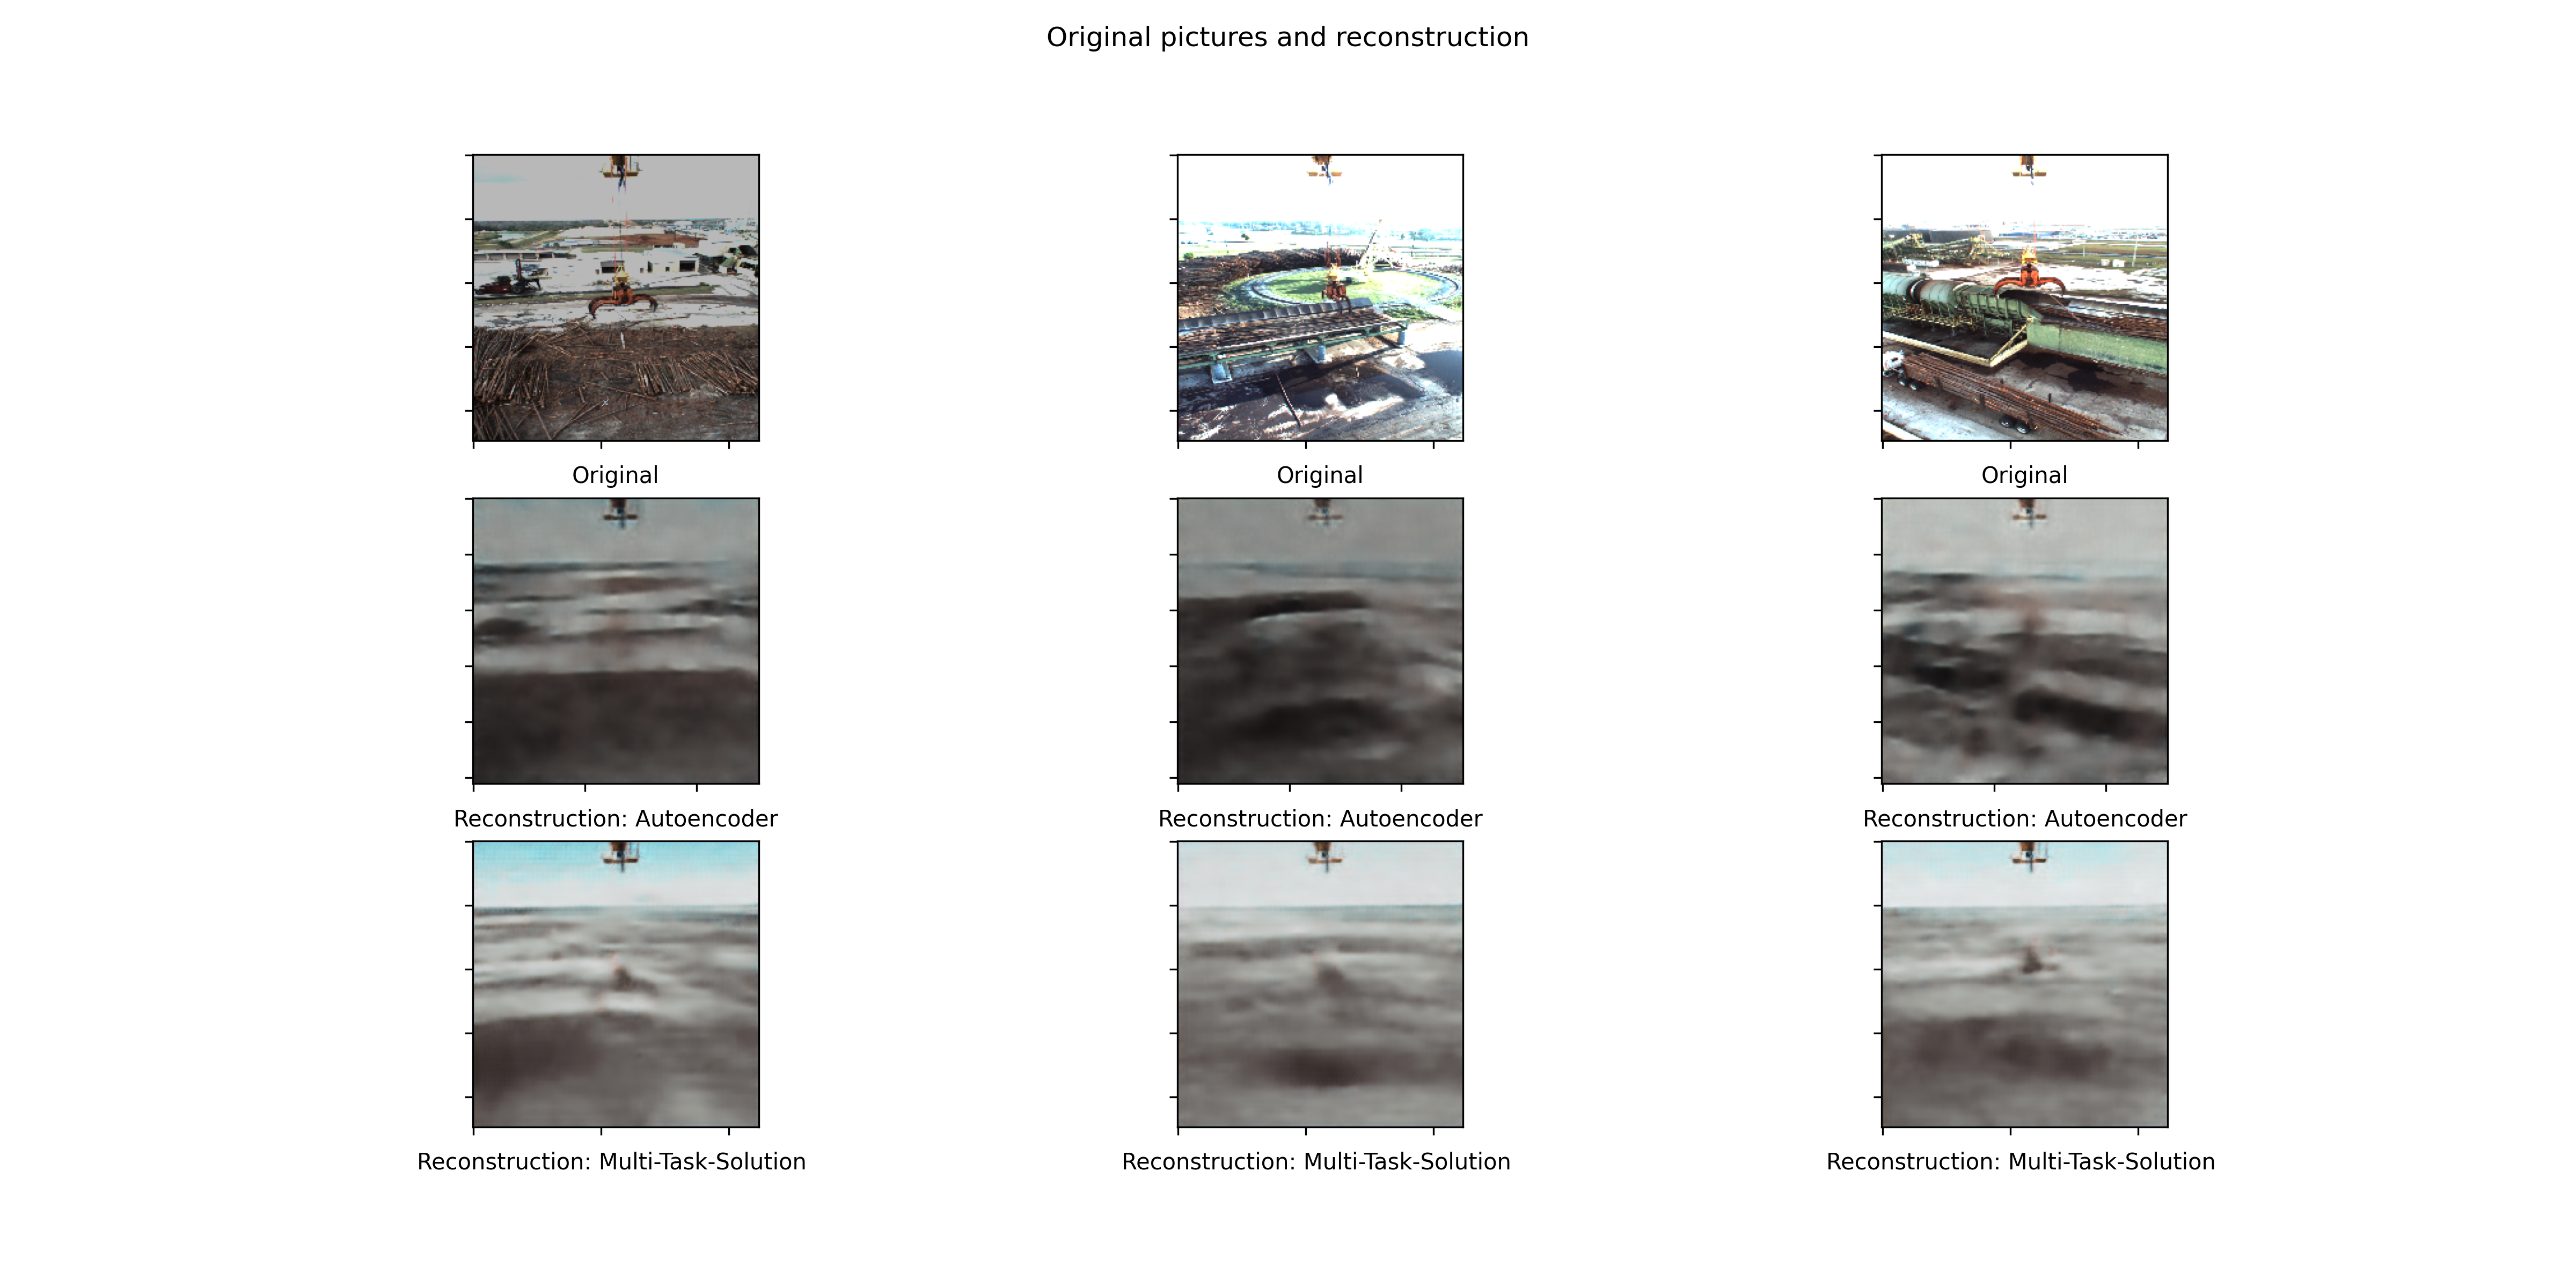
\includegraphics[width=1\textwidth, center]{bilder/Hauptteil/MT_Grapple/OriginalPicturesandReconstruction.png}
		\caption{Rekonstruktion - AE - MT}
		\label{img:RekonstruktionMTAE}
	\end{figure}  
	
	
	
	
	\section{Transferlernen und 'Greifer beladen?'-Klassifikation}
	\label{sec:TransferLearningGrappleLoaded}
	In vorangegangenen Kapitel wurde eine Repräsentation gefunden, welche die Merkmale des Greifer herausbildet. Ausgehend von dieser Repräsentation wird untersucht, ob ein Transfer auf weitere Aufgaben durchgeführt werden kann. Es wird der Ansatz des netzwerkbasierten tiefen Transferlernens genutzt um die Aufgabenstellung 'Greifer beladen?' zu lösen.
	\subsection{Werkzeug: TaskTransferOnAutoencoder}
	\label{sec:TransferSecondCriterionAutoenocder}		
	Als Quelldomäne wird ein Netzwerk, welches mittels \ac{tfae} erstellt wurde genutzt. In der Zieldomäne werden die Architektur und die Gewichte des Auteoncoder weiterverwendet. Der zweite Task wird durch eine neue Aufgabe ersetzt. Abbildung \ref{img:SchemaTTAE} zeigt das Schema des Ansatzes. 
	\begin{figure}[h]
		\centering
		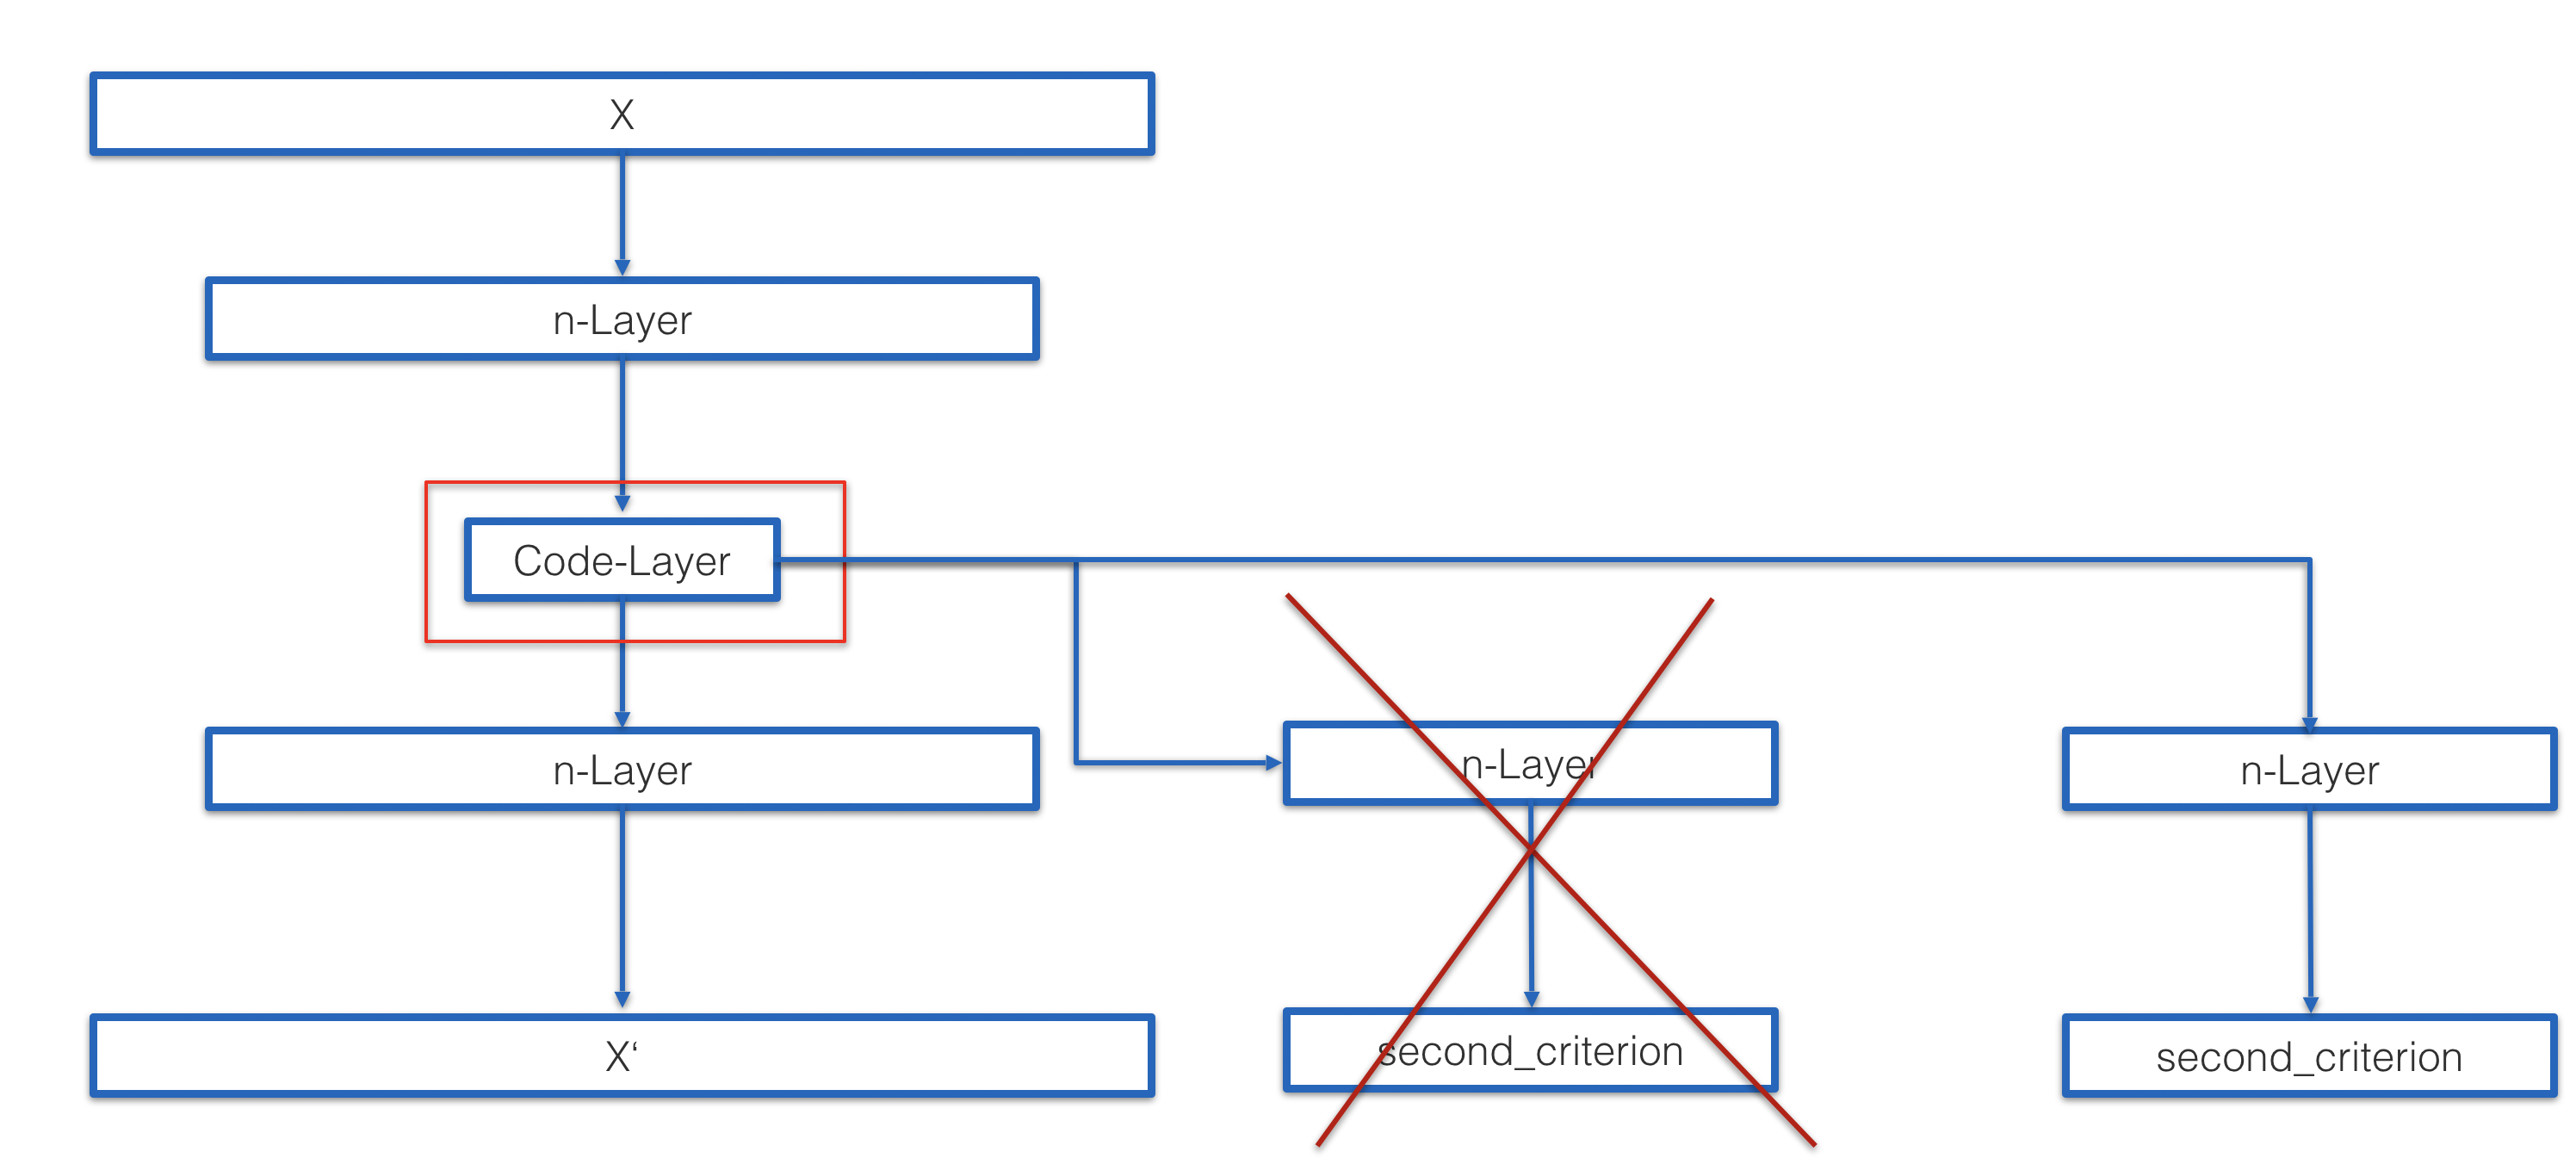
\includegraphics[width=0.6\textwidth, center]{bilder/Schema_Autoencoders/Schema_TSCAE.png}
		\caption[Schema TaskTransferOnAutoencoder]{Schema TaskTransferOnAutoencoder}
		\label{img:SchemaTTAE}
	\end{figure}
	Zur einfachen Anwendung des Ansatzes wurde ein Python-Modul mit der Klasse \acl{ttae} kurz \ac{ttae} erstellt. Abbildung \ref{img:KlassendiagrammTransferSecondCriterionAutoenocder} zeigt das zugehörige Klassendiagramm. Als Basis wird ein \ac{tfae} als Konstruktorargument übergeben. Die Parameter für den Autoencoder werden aus diesem Model kopiert. Zusätzlich müssen noch die Einstellungen für die zweite Aufgabe übergeben werden. Aus diesen beiden Teilen wird das neue Model erstellt. Die Parameter freeze\_encoder\_layers und freeze\_decoder\_layers ermöglichen es die Merkmalstransformation unverändert zu lassen. Es wird darüber gesteuert welche Schichten nicht neu trainiert werden können. 
	\begin{figure}[h]
		\centering
		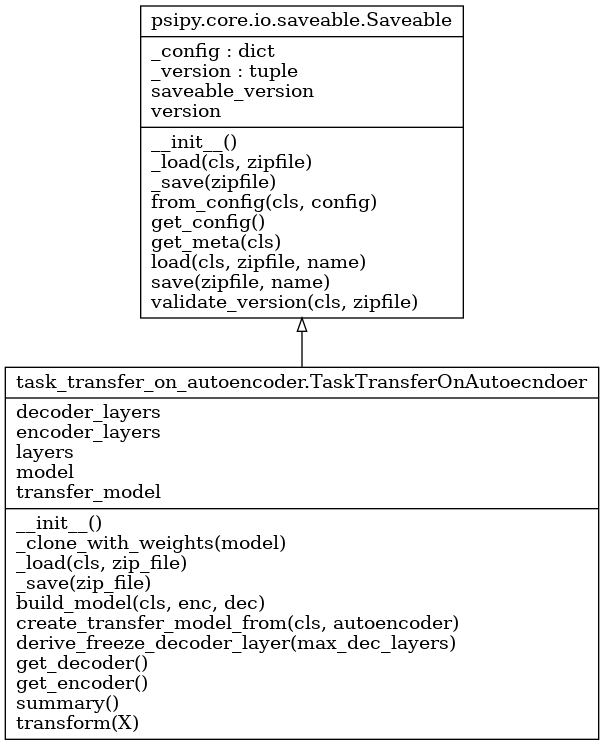
\includegraphics[width=0.5\textwidth, center]{bilder/Klassendiagramme/TTAE.png}
		\caption[Klassendiagramm TaskTransferOnAutoencoder]{Klassendiagramm TaskTransferOnAutoencoder}
		\label{img:KlassendiagrammTransferSecondCriterionAutoenocder}
	\end{figure}  
	Listing \ref{lst:BspTransferSecondCriterionAutoenocder} zeigt beispielhaft die Anwendung dieses Werkzeuges. Im Vergleich zu dem \ac{tfae} ist die Anwendung schon deutlich einfacher. Es gibt weniger Hyperparameter zum Modifizieren. Da das Modell auf einem trainierten \ac{tfae} basiert, ist kein $pretrain(..)$ mehr notwenig. Die Methode $fit(..)$ / $fit\_generator(..)$ wird auf dieselbe Weise wie in Keras angewendet.	
	
	\begin{lstlisting}[language=python,caption=Beispiel TransferSecondCriterionAutoenocder in Python, label=lst:BspTransferSecondCriterionAutoenocder]
	tscm = TransferLearningConvolutionalSecondCriterionAutoencoder(csc_autoencoder,
	second_criterion_topology=second_criterion_topology,
	second_criterion_loss = 'binary_crossentropy',                                                                                                   
	second_criterion_hidden_layer_kwargs = {'activation': 'relu'},
	second_criterion_output_layer_kwargs = {'activation': 'sigmoid'}, 
	loss_weights=[1, 0.01],
	freeze_encoder_layers = 2
	,freeze_decoder_layers =[0,1])
	
	history = tscm.fit(
	x_train,
	{"decoder": x_train, "second_criterion": y_train}, 
	epochs=1,
	batch_size = 128,
	validation_data=(x_test,{"decoder": x_test, "second_criterion": y_test}))
	)
	\end{lstlisting}	
	
	\subsection{Experiment}
	\label{subsec:TransferLogs}
	In \ref{sec:MultiTaskGreifererkennung} wurde ein fokussiertes Embedding erstellt. Zur Überprüfung, ob ausgehend von dieser Lösung, neue Aufgaben gelöst werden können wird ein Transfer auf die Aufgabe 'Greifer beladen?' durchgeführt. Dabei kommt der gerade vorgestellte Ansatz zum Einsatz.  
	
	Mit dem vorgestellten Ansatz lässt sich die Aufgabe 'Greifer beladen?' lösen. Im Median von drei Versuchen wird ein Accuracy von 0.9827\% erreicht, was nahezu der Leistung der Basislinie mit einer Accuracy von 0.9828\% entspricht. In Abbildung \ref{img:Ergebnis_Transfer} sind die Ergebnisse des Versuchs dargestellt. Die Unterabbildung \ref{img:Einbettung_Logs_Vorhersage} stellt die neu gefundene Einbettung dar. Die blauen Datenpunte entsprechen der Vorhersage True Positiv, die lila Datenpunkte der Vorhersage True Negativ, gelb entspricht False Positiv und grün False Negativ. Es ist eine deutliche Anpassung der Einbettung an die Problemstellung erkennbar, wobei der Übergang von der einen zur anderen Klasse nicht 100\% korrekt ist. Der erfolgreiche Transfer zeigt, dass das die Fokussierung des Basis-Autoencoders erfolgreich ist.     

		 \begin{figure}[h]
			\centering
			\begin{subfigure}[c]{0.49\textwidth}			
				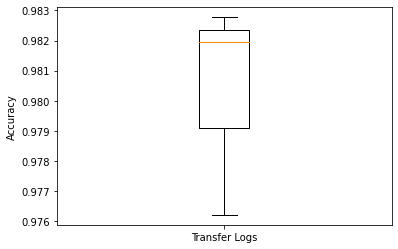
\includegraphics[width=1\textwidth,center]{bilder/Hauptteil/Transfer_Logs/Acc_Transfer_Logs.png}
				\caption{Accuracy}
				\label{img:AccuracyTransferLogs}	
			\end{subfigure}
			\begin{subfigure}[c]{0.49\textwidth}			
				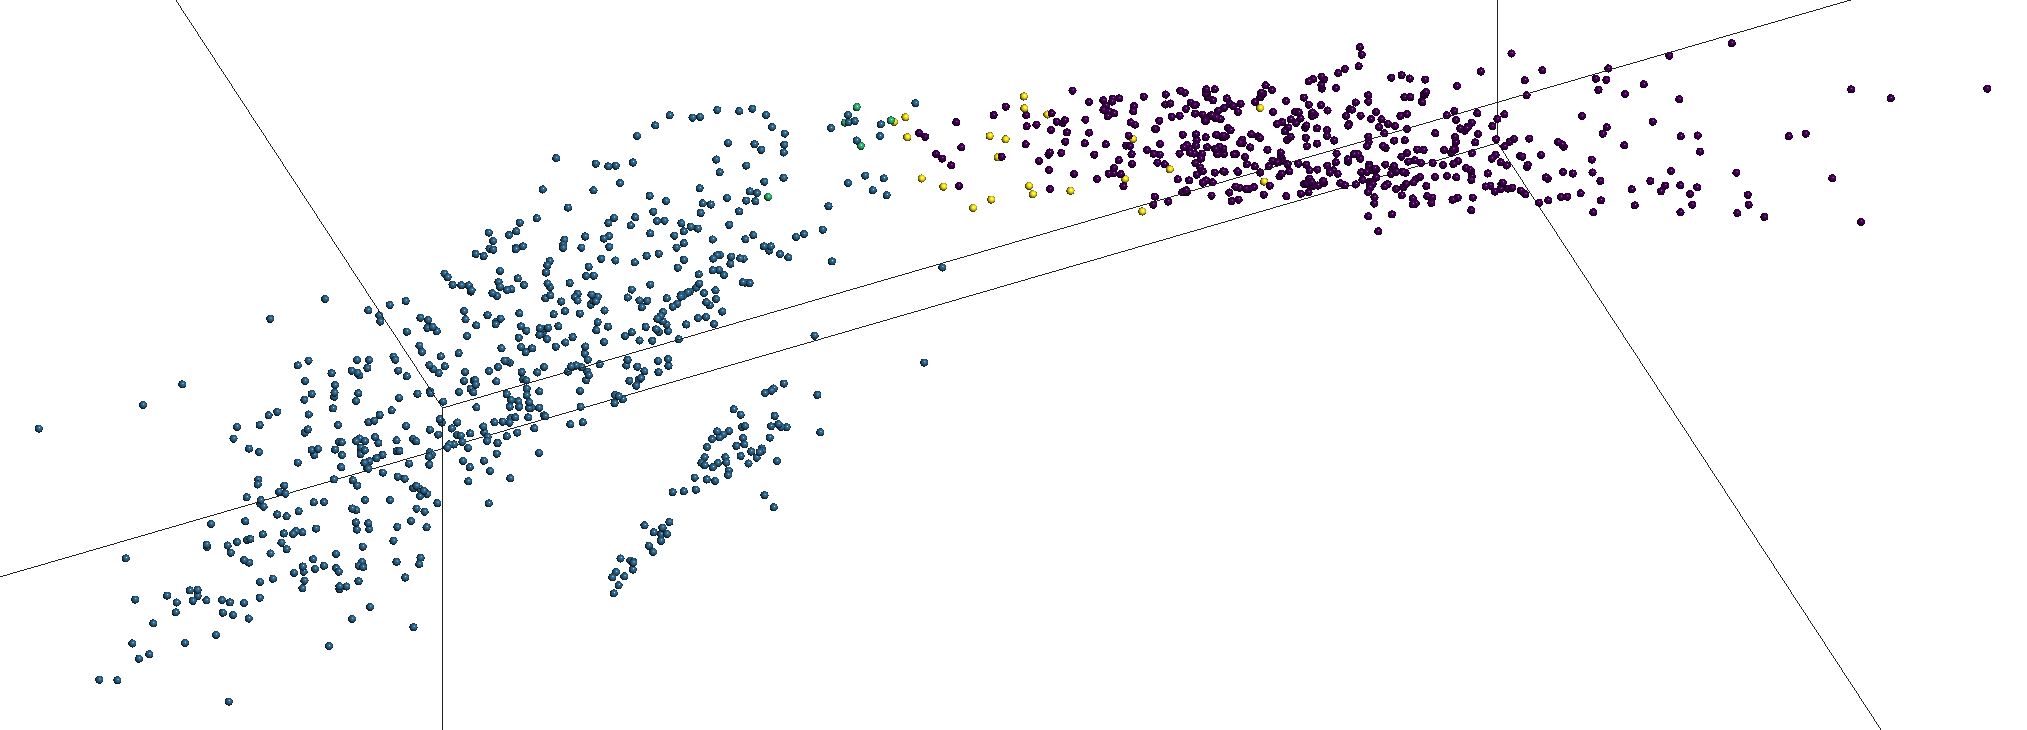
\includegraphics[width=1\textwidth, center]{bilder/Hauptteil/Transfer_Logs/Logs_transfer_emb.png}
				\caption{Einbettung mit Vorhersage}
				\label{img:Einbettung_Logs_Vorhersage}	
			\end{subfigure}
			\caption{Ergebnis Transfer}
			\label{img:Ergebnis_Transfer}
		\end{figure}
		
	\section{AutoML und 'Greifer beladen?'}
	\label{sec:Transfer_autoMl}
	Die starke Anpassung an die Klassifikationsaufgabe im vorangegangenen Versuch motiviert einen Blick auf die Hyperparameter zur Gewichtung der Verlustfunktion zu werfen. Ziel dieses Versuches ist es, herauszufinden welchen Einfluss die Hyperparameter auf das Ergebnis hat. Es gibt sehr viele Möglichkeiten für die Gewichtung der Verlustfunktion. Um den manuellen Aufwand für weitere Anwendungen gering zu halten, wird ein neues Modul erstellt, welches auf \ac{automl} zur Hyperparameteroptimierung zurückgreift.
	\subsection{Werkzeug: AutoTaskTransferOnAutoencoder}
	\label{subsec:AutoTaskTransferOnAutoencoder}
	Das neue Modul integriert den Ansatz in der Klasse \acl{autottae}, kurz \ac{autottae}. Sie integriert die Klasse \acl{ttae} und erweitert sie mithilfe des HpBandSter-Frameworks um \ac{automl}-Ansätze zur \ac{hpo}. Konkret erbt die Klasse von hpbandster.core.worker. Zur Speicherung und Verwaltung der Hyperparameter wird auf die Klasse HyperparameterMixin zurückgegriffen. Nach nach dem Instanziieren der Klasse können weitere sinnvolle Hyperparameter gesetzt werden.
	In Abbildung \ref{img:KlassendiagrammAutoTaskTransferOnAutoencoder}  ist das zugehörige Klassendiagramm abgebildet. 
	\begin{figure}[h]
		\centering
		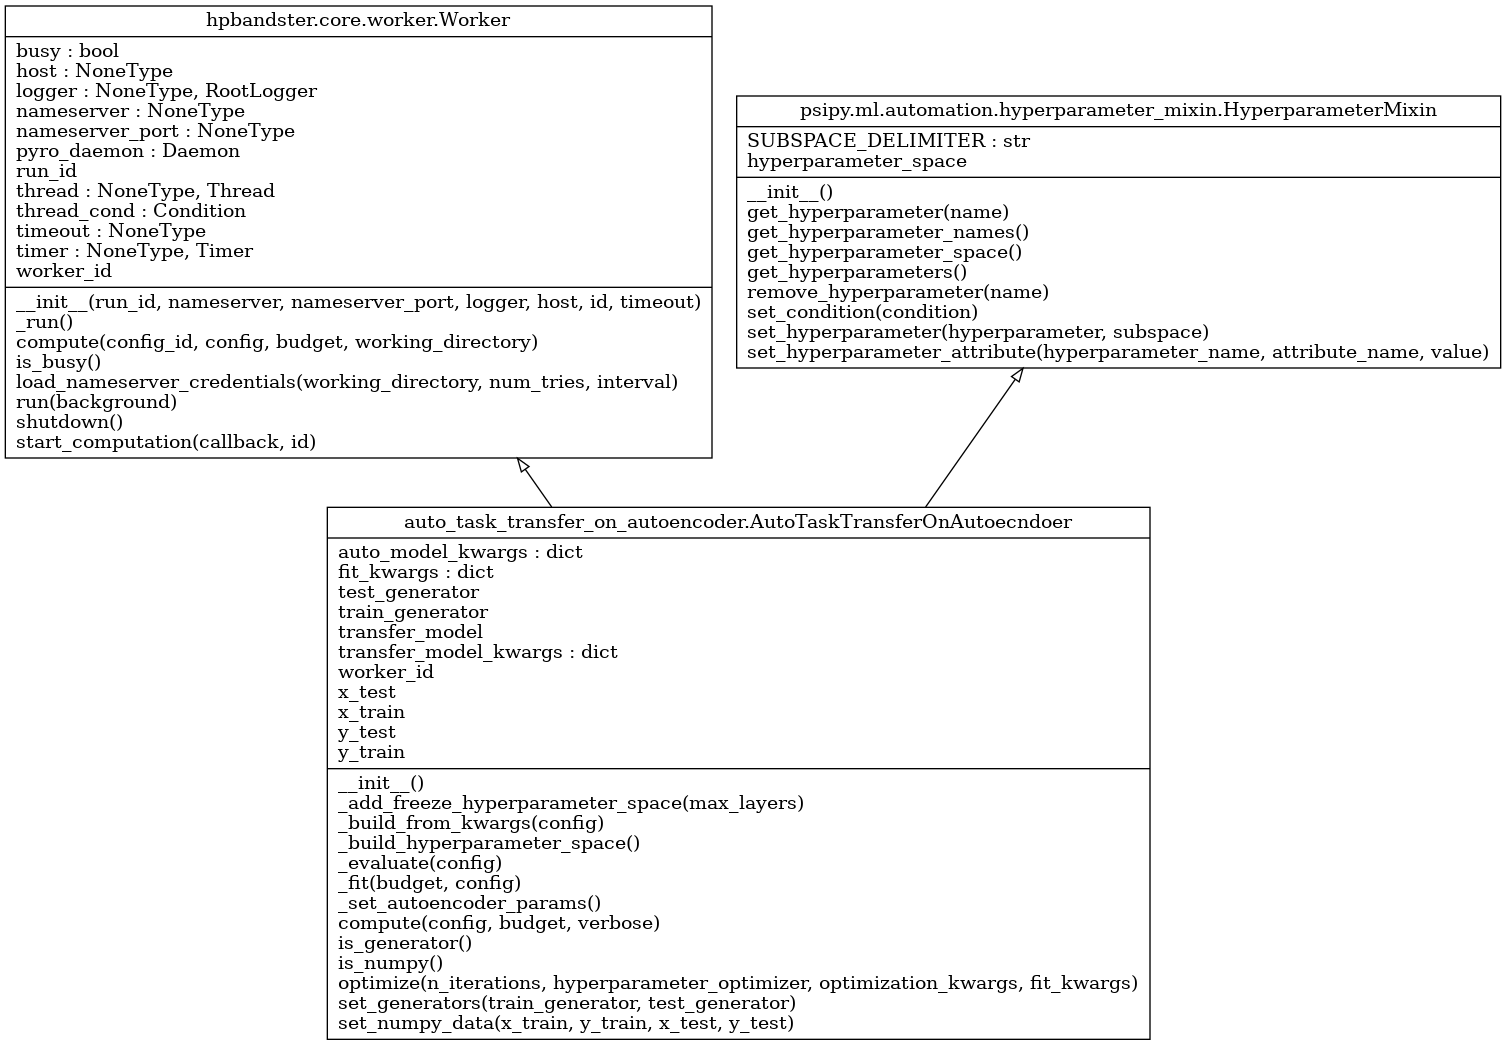
\includegraphics[width=1\textwidth, center]{bilder/Klassendiagramme/AutoTTAE.png}
		\caption[Klassendiagramm AutoTaskTransferOnAutoencoder]{Klassendiagramm AutoTaskTransferOnAutoencoder}
		\label{img:KlassendiagrammAutoTaskTransferOnAutoencoder}
	\end{figure}  
	In Listing \ref{lst:BspAutoTransferSecondCriterionAutoenocder} ist eine einfache Implementierung eines AutoTaskTransferOnAutoencoder dargestellt. Der Konstruktor unterscheidet sich nur an einer Stelle zum Konstruktor des TaskTransferOnAutoencoder. Es wird keine Instanz des SCAE übergeben, sondern ein Pfad zu einem abgespeicherten Modell eines SCAE. 
	Im Gegensatz zur bisherigen Vorgehensweise werden die Trainings und Testdaten mit der Methode $set\_generators(..)$  oder $set\_numpy\_data(..)$ übergeben. Ziel ist es dabei die Komplexität der Methode $optimize(..)$ zu reduzieren. Durch den Aufruf von $optimize(..)$, wird der Optimierungsvorgang gestartet. Die Parameter sind dabei die Anzahl an Iterationen, die Optimierungsstrategie und ein Wörterbuch, welches zusätzliche Einstellungen für die einzelnen Optimierer enthalten kann. In jeder Iteration der Optimierung wird ein neuer TaskTransferOnAutoencoder erstellt und mittels der ausgewählten Hyperparameter und übergebenen Daten trainiert. 
	\begin{lstlisting}[language=python,caption=Beispiel AutoTransferSecondCriterionAutoenocder in Python, label=lst:BspAutoTransferSecondCriterionAutoenocder]
	tscm = AutoTransferConvolutionalSecondCriterionAutoencoder(max_deep_freeze=2,
	path_to_model = path_to_base_model,            
	second_criterion_topology=second_criterion_topology,
	second_criterion_loss = 'categorical_crossentropy',                                                                                                   
	second_criterion_hidden_layer_kwargs = {'activation': 'relu'},
	second_criterion_output_layer_kwargs = {'activation': 'softmax'},
	second_criterion_metrics = {'second_criterion':'accuracy'}
	)
	
	tscm.set_generators(train_datagenerator,test_datagenerator)
	
	
	best_config, history = tscm.optimize(3
	,'RandomSearch'
	,optimization_kwargs = optimization_kwargs)
	\end{lstlisting}
	Das Werkzeug unterstützt derzeit die Optimierer, Zufallssuche, Hyperband und BOHB. Der vom Framework bereitgestellte Parameter Budget wird zur Festlegung der Epochen eingesetzt. Um ein Overfitting zu verhindern, wird ein EarlyStopping Kriterium eingesetzt. 
	Besondere Beachtung muss die Evaluationsmetrik zur Bewertung eines Optimierungslaufes finden. Da ein zu optimierender Hyperparameter die Gewichtung der Verlustfunktion ist, muss dies bei dem Einsatz der Evaluationsmetrik berücksichtigt werden. Die Evaluationsmetrik kann bei dem Erstellen der Klasse frei gewählt werden.
	
	\subsection{Experiment}
	\label{subsec:AutoMLExperiment}
	In diesem Versuch wird die selbe Ausgangslage wie im Vorangegangenen Versuch genutzt. Der Unterschied besteht darin, dass der Hyperparameter 'Gewichtung der Verlustfunktion' automatisch gesucht wird. Zur Bewertung eines Optimierungsdurchlaufs wird der Wert $1-Accuracy$ des finalen Modells herangezogen. Die Ergebnisse von drei Optimierungsdurchläufen mit jeweils drei Iterationen sind in Anhang \ref{appendix:AutoML} zu finden. In den finalen Ergebnissen für die Aufgabe 'Greifer beladen?' erreichen alle drei Versuch mindestens eine Accuracy von 0.98\% bei verschiedenen Gewichtungen.  Wirft man einen Blick auf die Durchläufe mit vollem Budget von 15 ist in Versuch [2,0,1] \ref{lst:AutoML2c} zu sehen, dass die Accuracy deutlich auf 0,79\% abfällt. In Abbildung \ref{img:EmbeddingAutoMLTransfer} sind die Einbettungen der drei Optimierungsdurchläufe abgebildet. Die Einzelnen Datenpunkte sind entsprechend ihrer Klasse eingefärbt. Es ist in allen drei Fällen eine Anpassung an die Klassifizierungsaufgabe erkennbar. In Durchlauf drei \ref{img:AutoMLEinbettungV3} ist die Anpassung deutlich geringer als in den anderen beiden Durchläufen. Der Versuch [2,0,1] und die Einbettung drei liefern deutliche Hinweise, dass die Gewichtung der beiden Teile der Verlustfunktion einen starken Einfluss auf die Modellqualität haben. 
	
	\begin{figure}[h]
		\centering
		\begin{subfigure}[c]{0.32\textwidth}			
			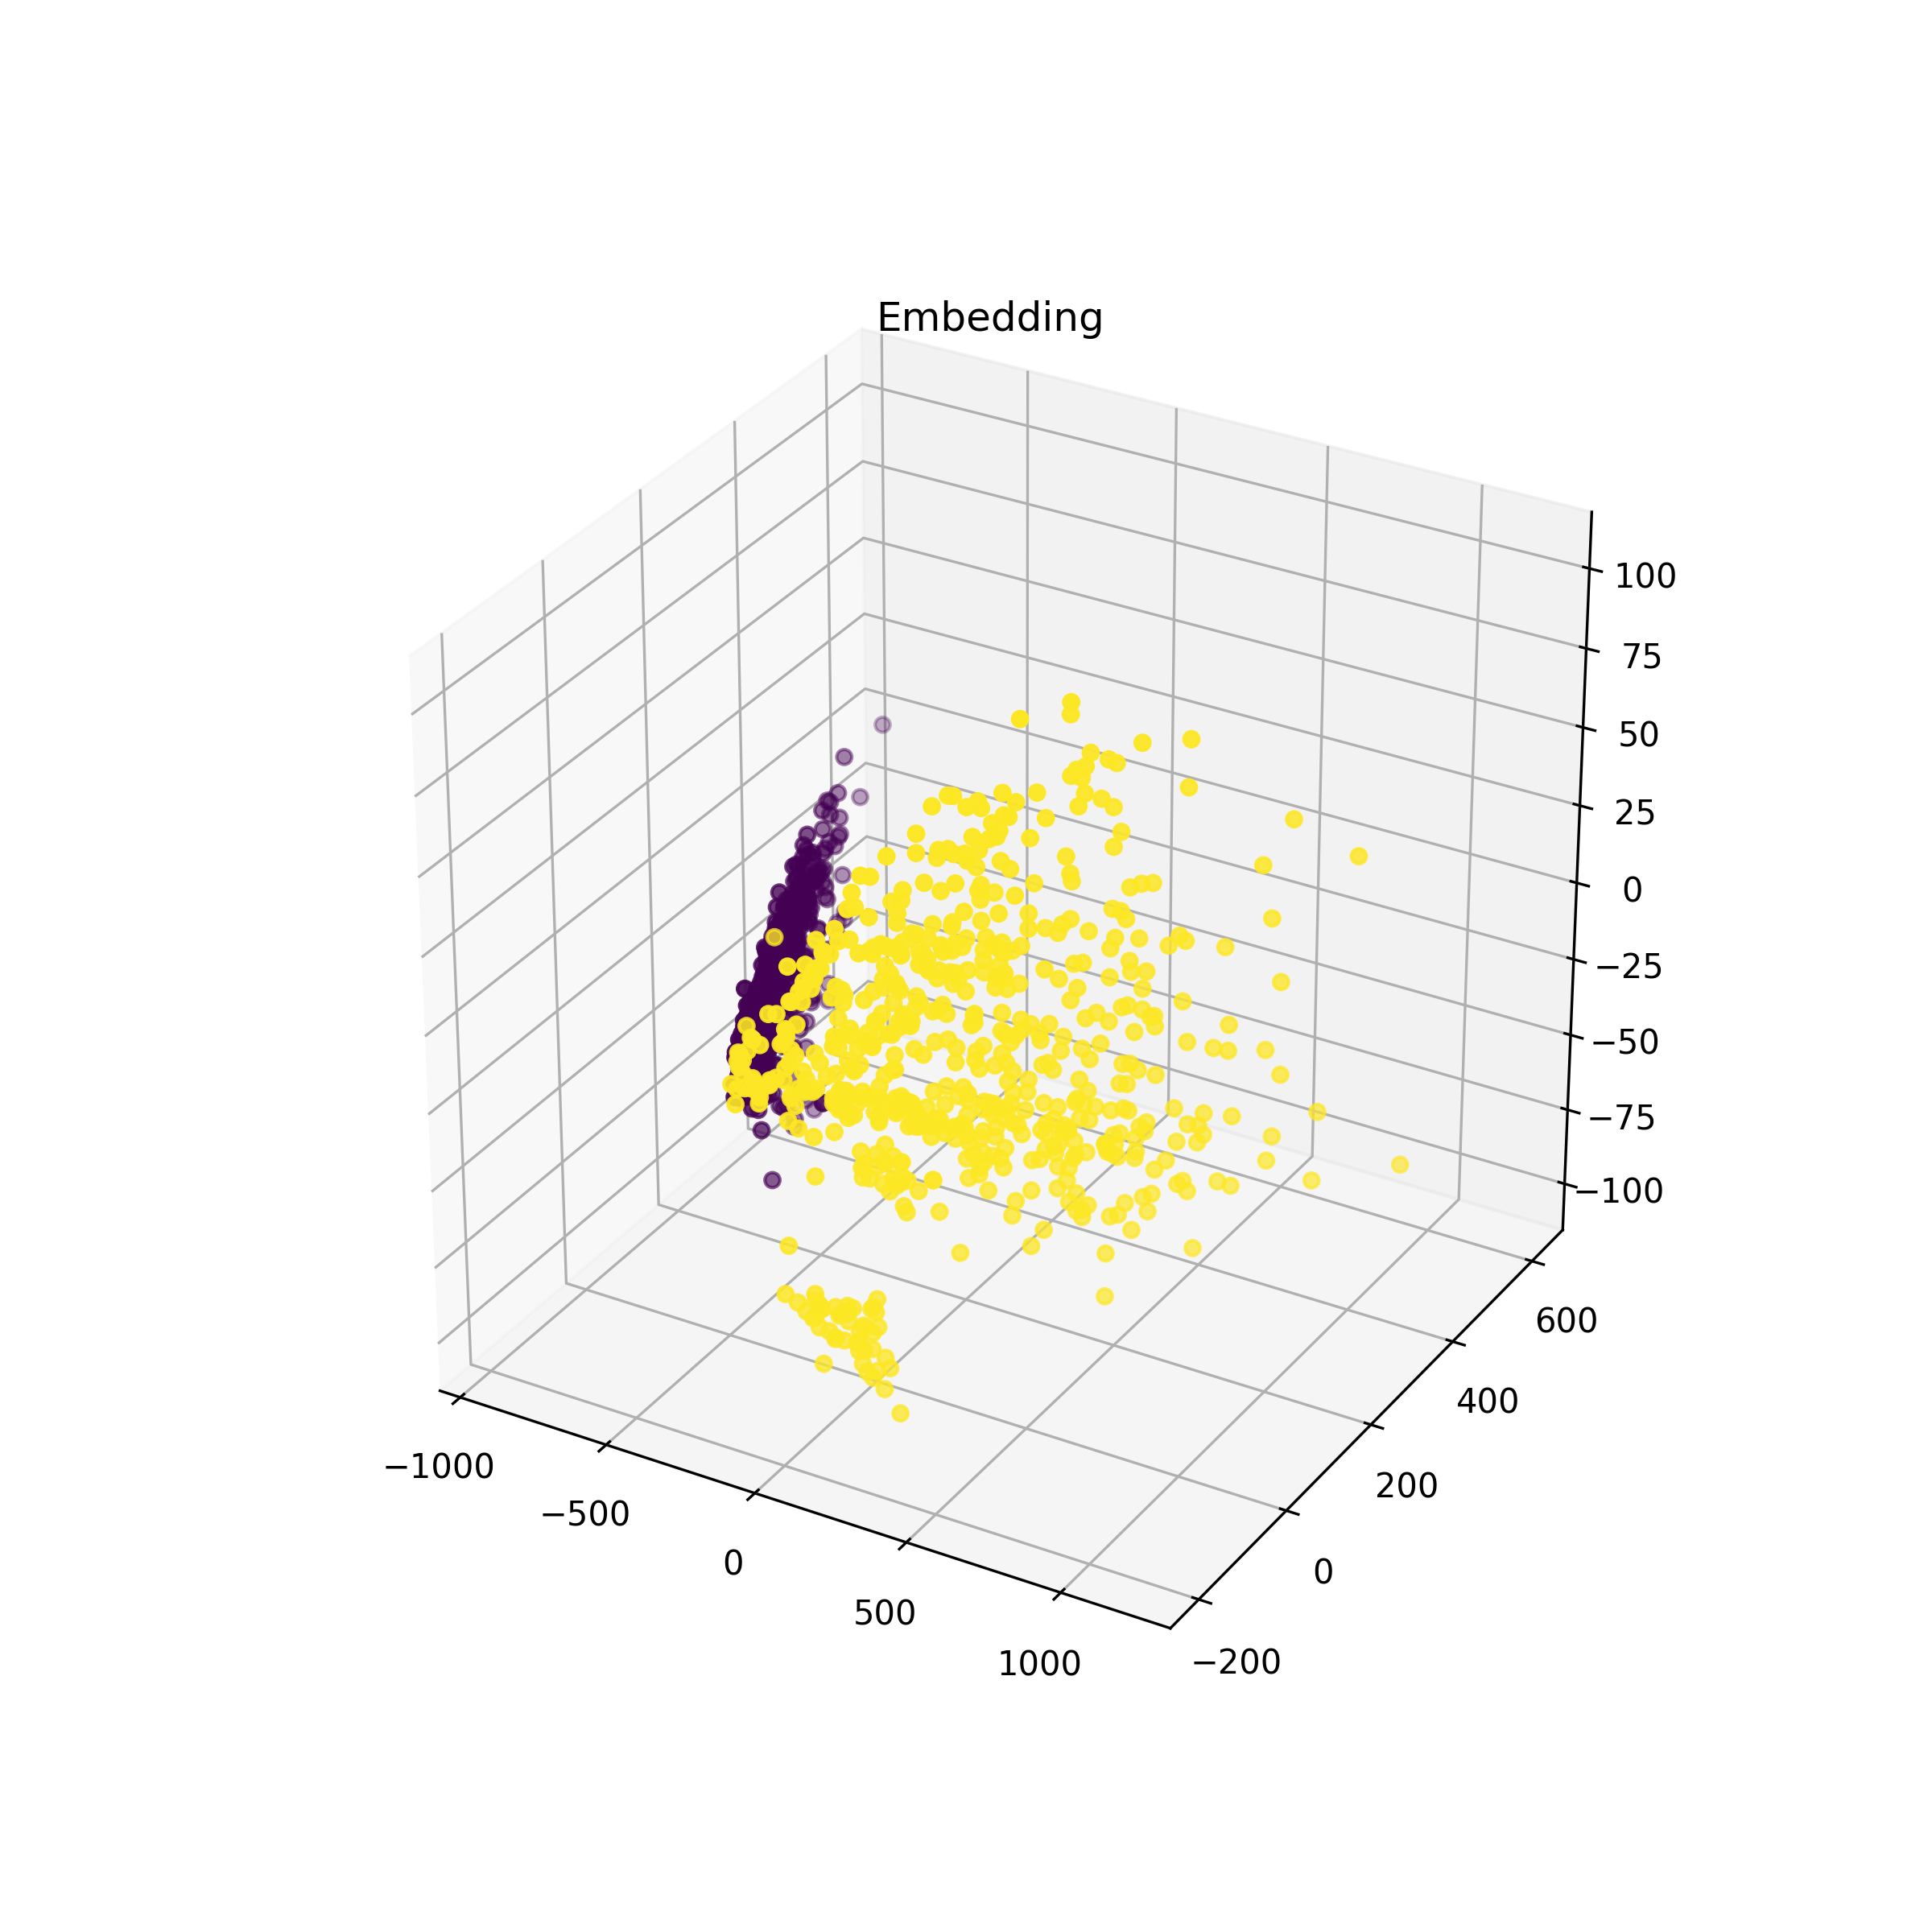
\includegraphics[width=1\textwidth,center]{src/AutoML/1/Embedding.png}
			\caption{Einbettung 1}
			\label{img:AutoMLEinbettungV1}	
		\end{subfigure}
		\begin{subfigure}[c]{0.32\textwidth}			
			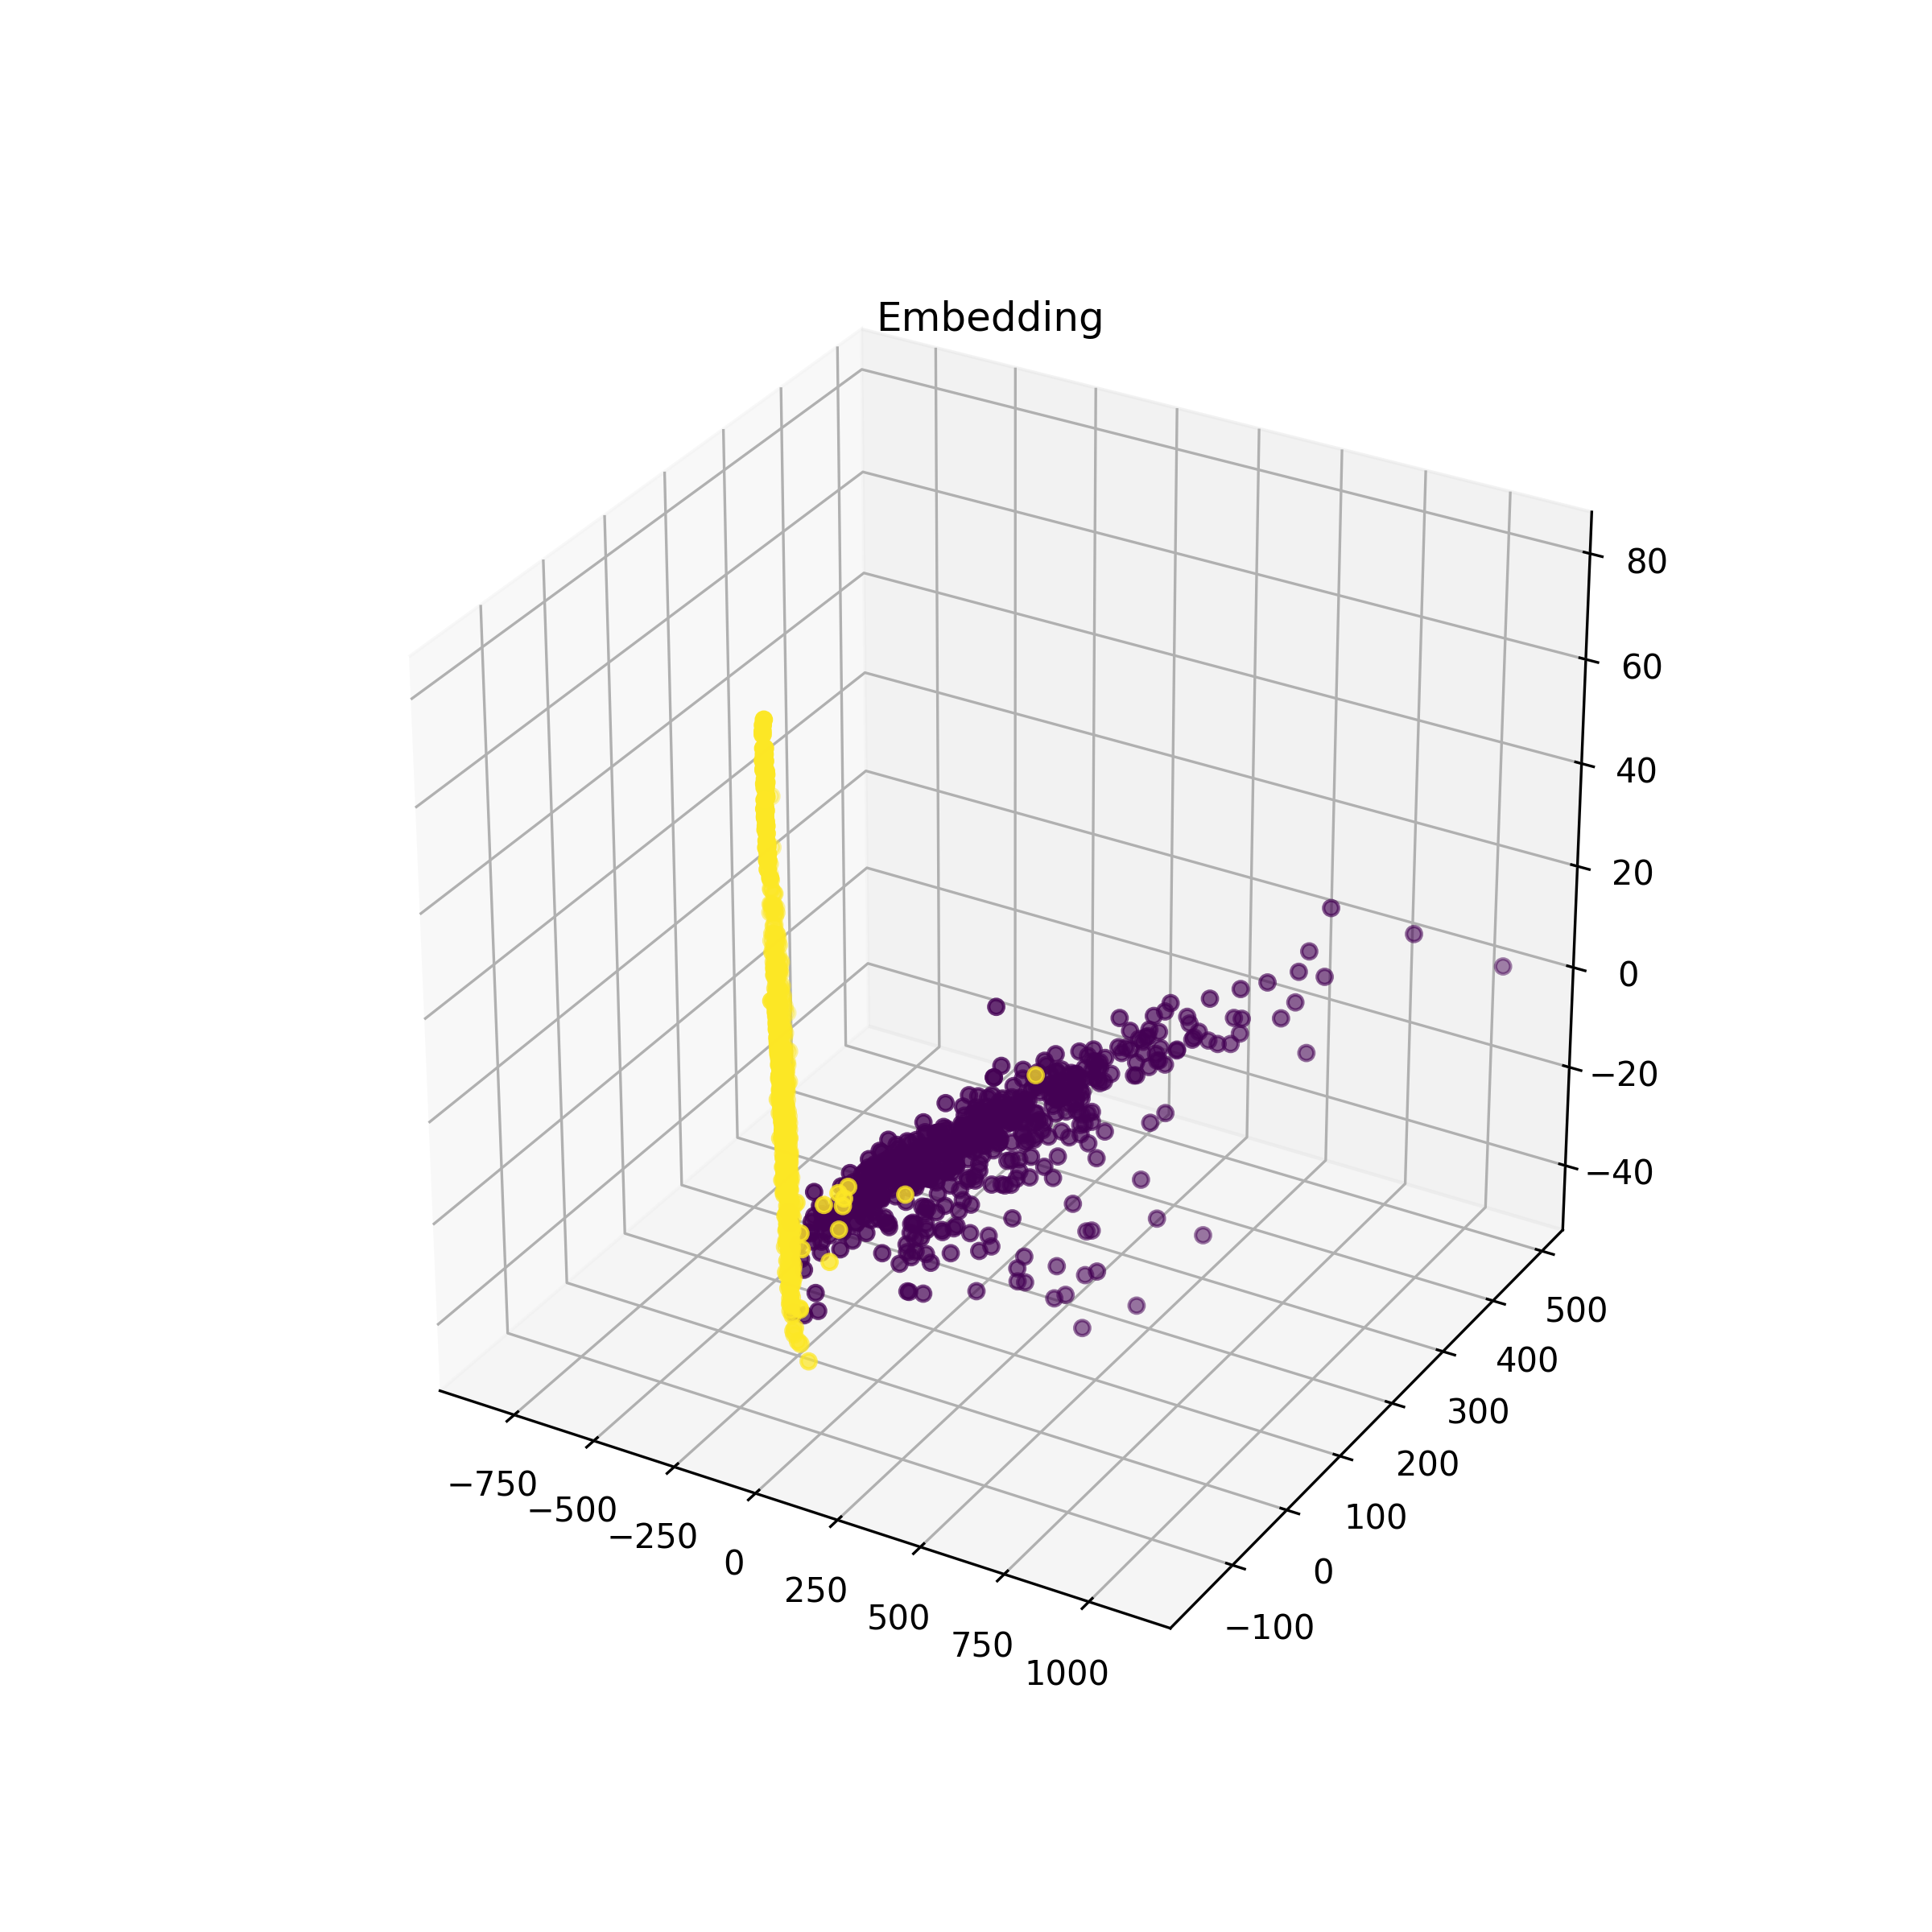
\includegraphics[width=1\textwidth, center]{src/AutoML/2/Embedding.png}
			\caption{Einbettung 2}
			\label{img:AutoMLEinbettungV2}	
		\end{subfigure}
		\begin{subfigure}[c]{0.32\textwidth}			
			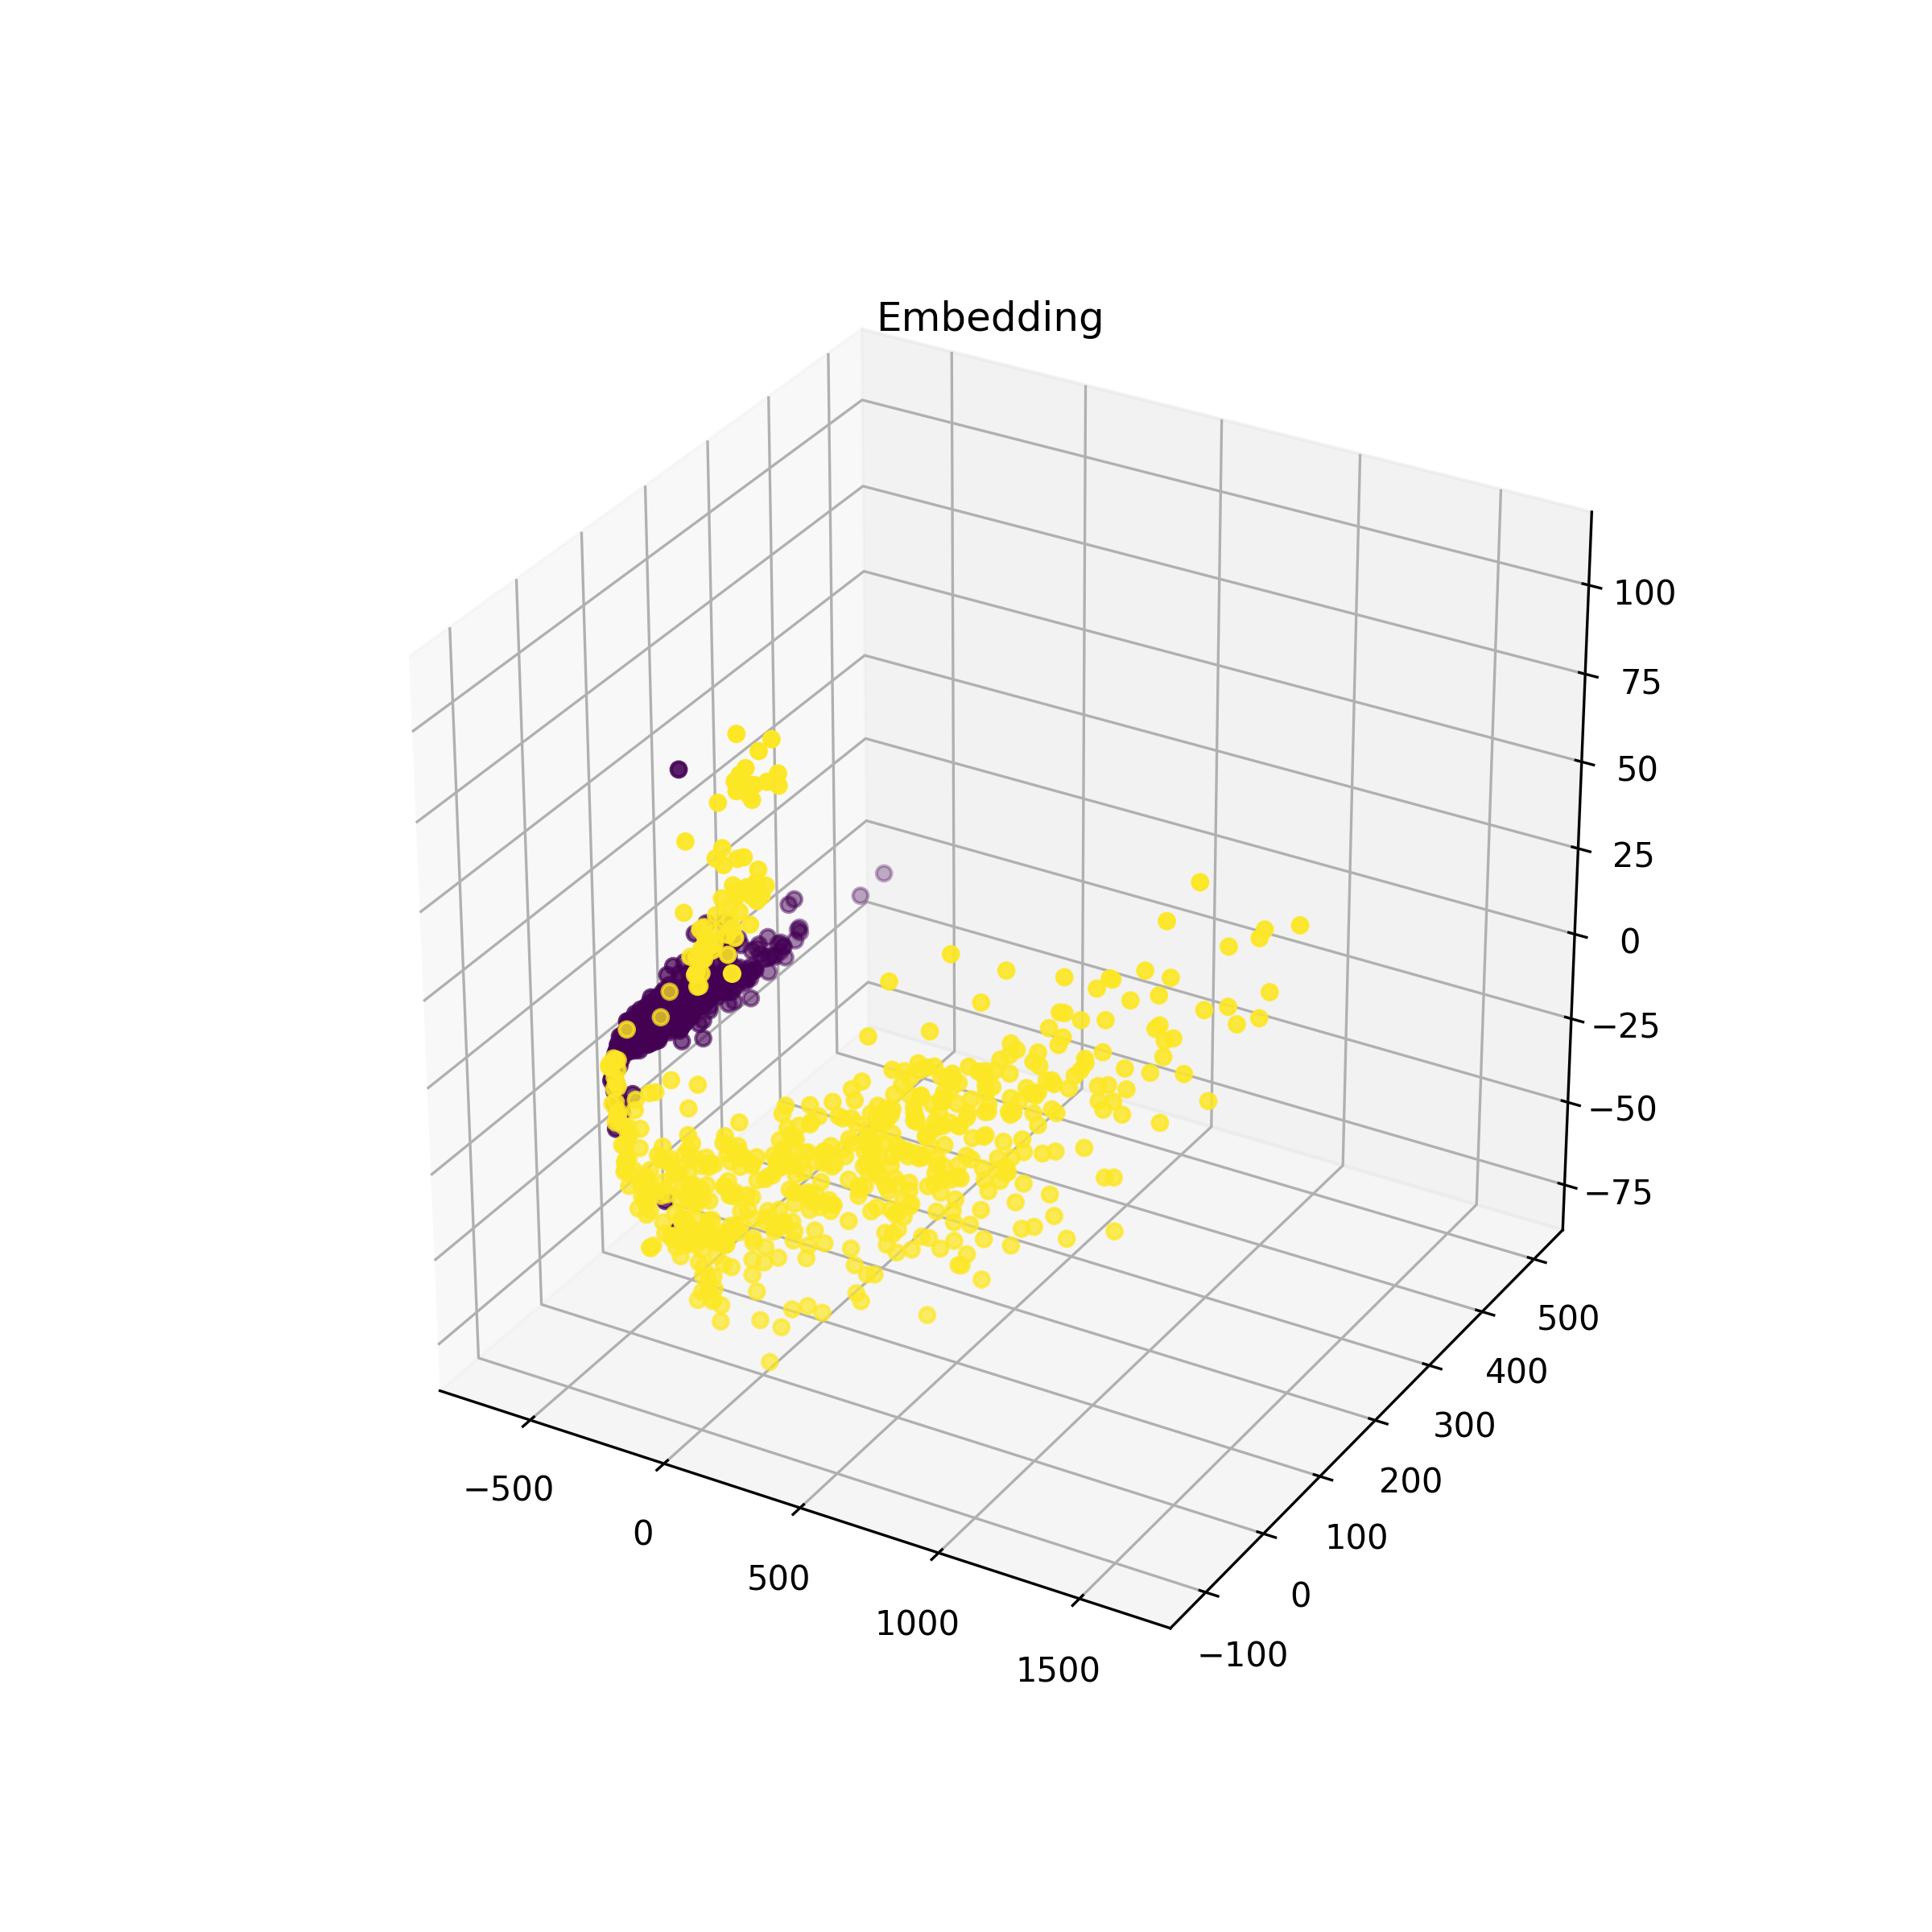
\includegraphics[width=1\textwidth, center]{src/AutoML/3/Embedding.png}
			\caption{Einbettung 3}
			\label{img:AutoMLEinbettungV3}	
		\end{subfigure}
		\caption{Einbettungen AutoML-Transfer}
		\label{img:EmbeddingAutoMLTransfer}
	\end{figure}
	
	
	\section{Datenmenge und 'Greifer beladen?'}
	\label{sec:TransferDatenmenge}
	In den bisherigen Experimenten wurde die Grundsätzliche Funktionalität der Ansätze untersucht. Besonderes  Kosten-Einsparungspotential besteht bei einem Einsatz von geringeren Datenmengen. In diesem Versuch wird untersucht wie sich die Lösung bei unterschiedlichen Datenmengen verhält. Es wird untersucht, wie sich die Leistung der Ansätze bei 200, 2000 und 9749 annotierten Daten verhält. Als Gewichtungsfaktor der Verlustfunktion werden die Hyperparameter von Versuch [2, 0, 2] \ref{appendix:AutoML} 2 genutzt. 
	
	In Abbildung \ref{img:VergleichDatenmenge} sind die Ergebnisse des Versuchs für die Aufgabe ist der Greifer beladen dargestellt. Auf der X-Achse sind die Datenmengen, auf der y-Achse die Accuracy dargestellt. Der Versuch wurde einmal als \ac{ttae}-Ansatz hier blau und einmal als \ac{tfae}-Ansatz (lila) durchgeführt. Bei allen drei Datenmengen erreicht der \ac{ttae}-Ansatz deutlich bessere (22\%,15\%,5\%) Ergebnisse. Insbesondere bei niedrigen Datenmengen erzielt der \ac{ttae}-Ansatz gute Ergebnisse. Bei 2000 Bildern ist die Accuracy nur 2\% schlechter als die Basislinie. Die Einzelergebnisse sind in Abbildung \ref{img:DatenmengenLeistung} dargestellt.   
	
	\begin{figure}[h]
		\centering
		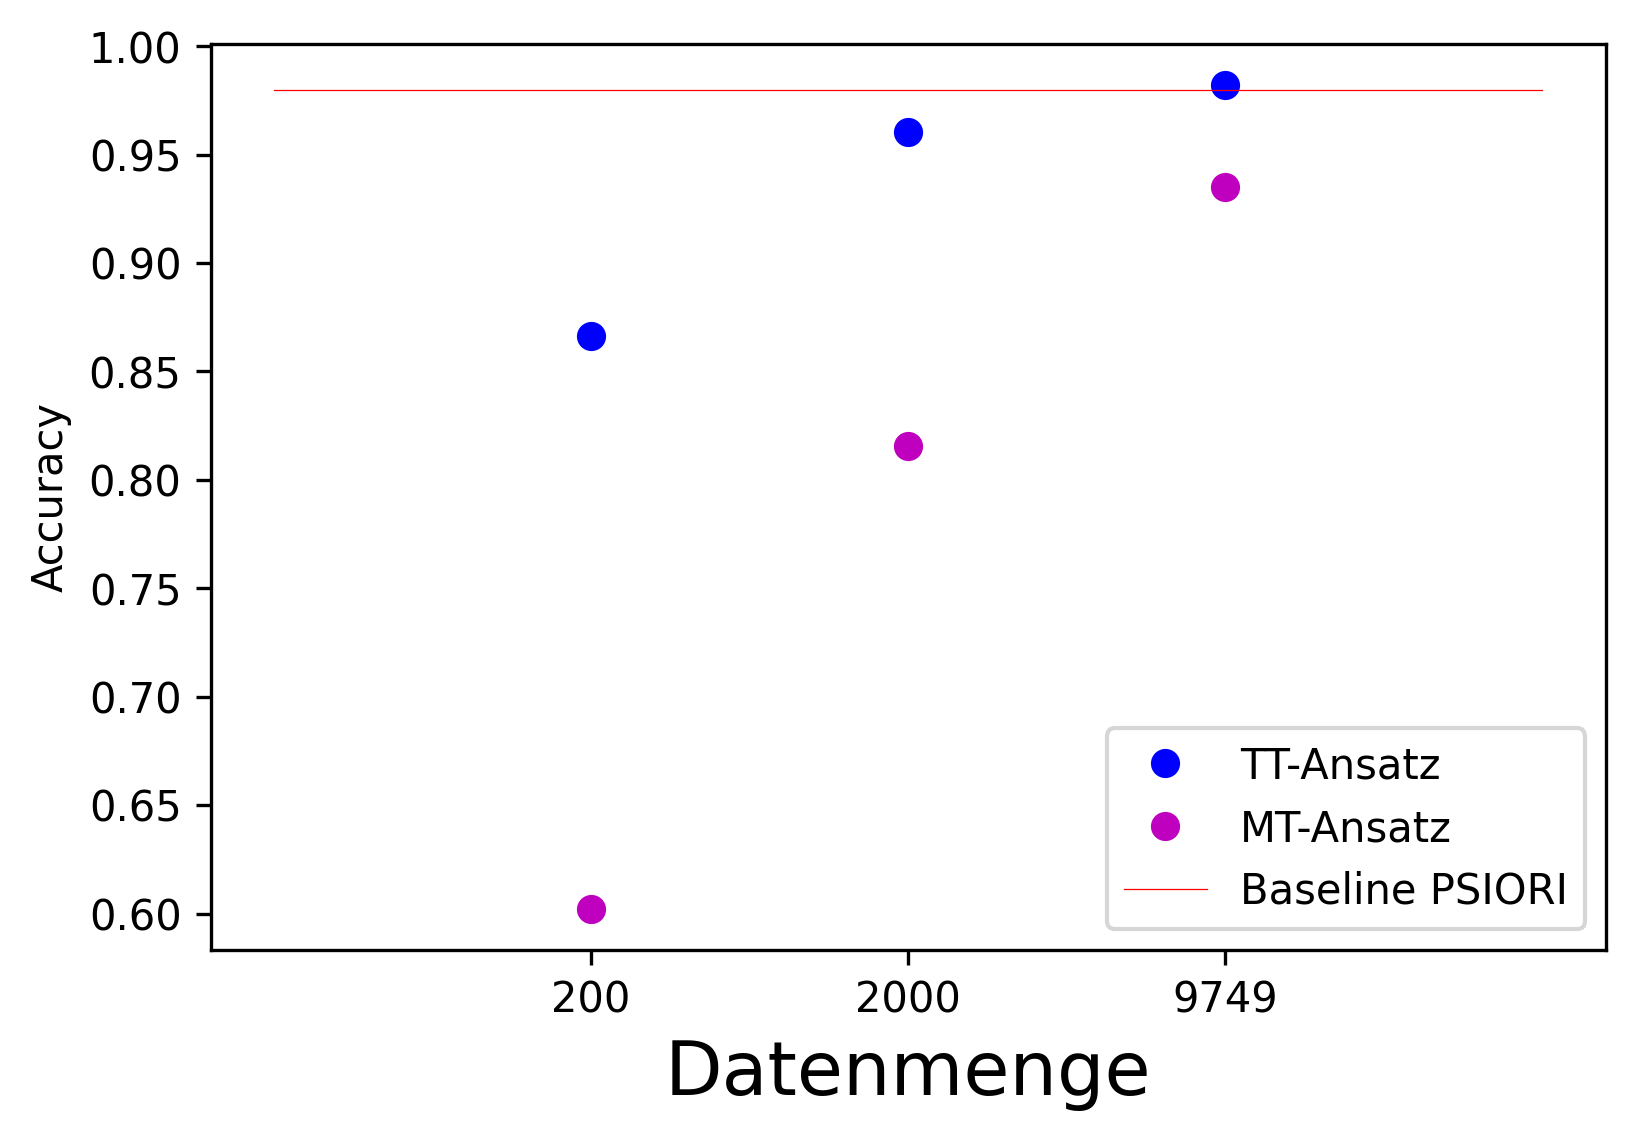
\includegraphics[width=1\textwidth, center]{bilder/Hauptteil/Transfer_Logs_Datenmenge//Acc_compare_Logs_data.png}
		\caption{Vergleich-Ansätze Datenmenge}
		\label{img:VergleichDatenmenge}
	\end{figure}  
	
	\begin{figure}[h]
		\centering
		\begin{subfigure}[c]{0.49\textwidth}			
			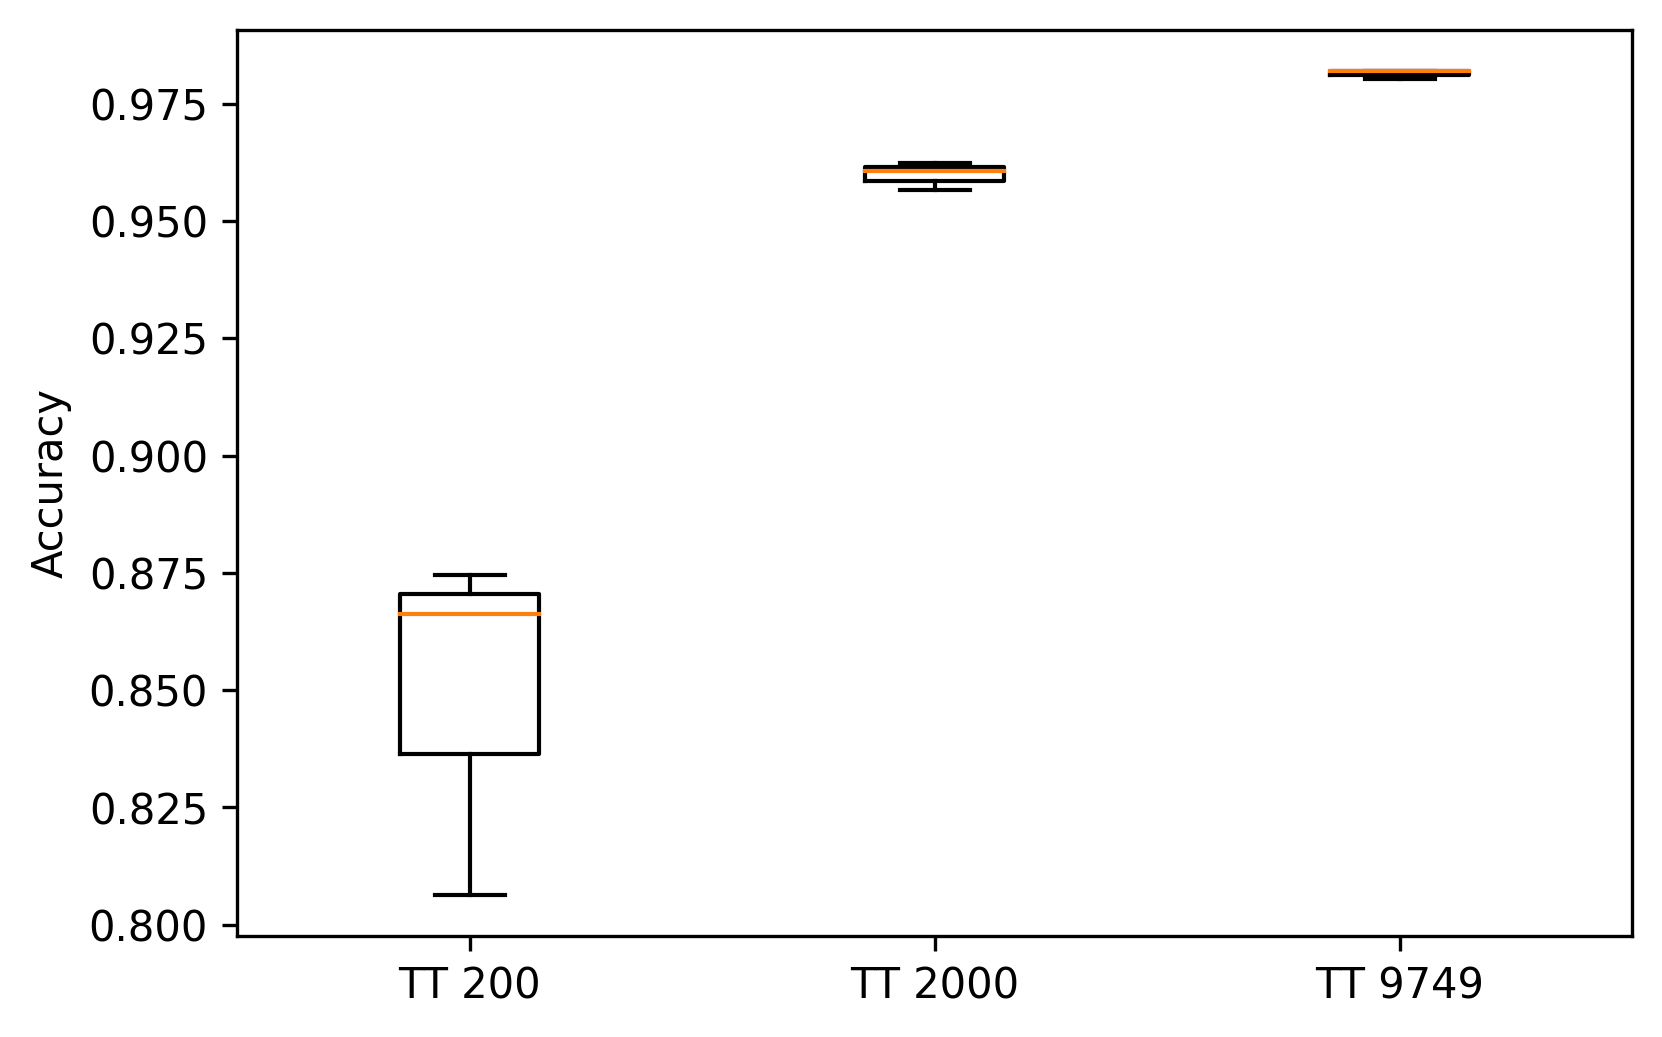
\includegraphics[width=1\textwidth,center]{bilder/Hauptteil/Transfer_Logs_Datenmenge/Acc_Transfer_Logs_data.png}
			\caption{TTAE Accuracy Datenmenge}
			\label{img:TT_ACC_DATA}	
		\end{subfigure}
		\begin{subfigure}[c]{0.49\textwidth}			
			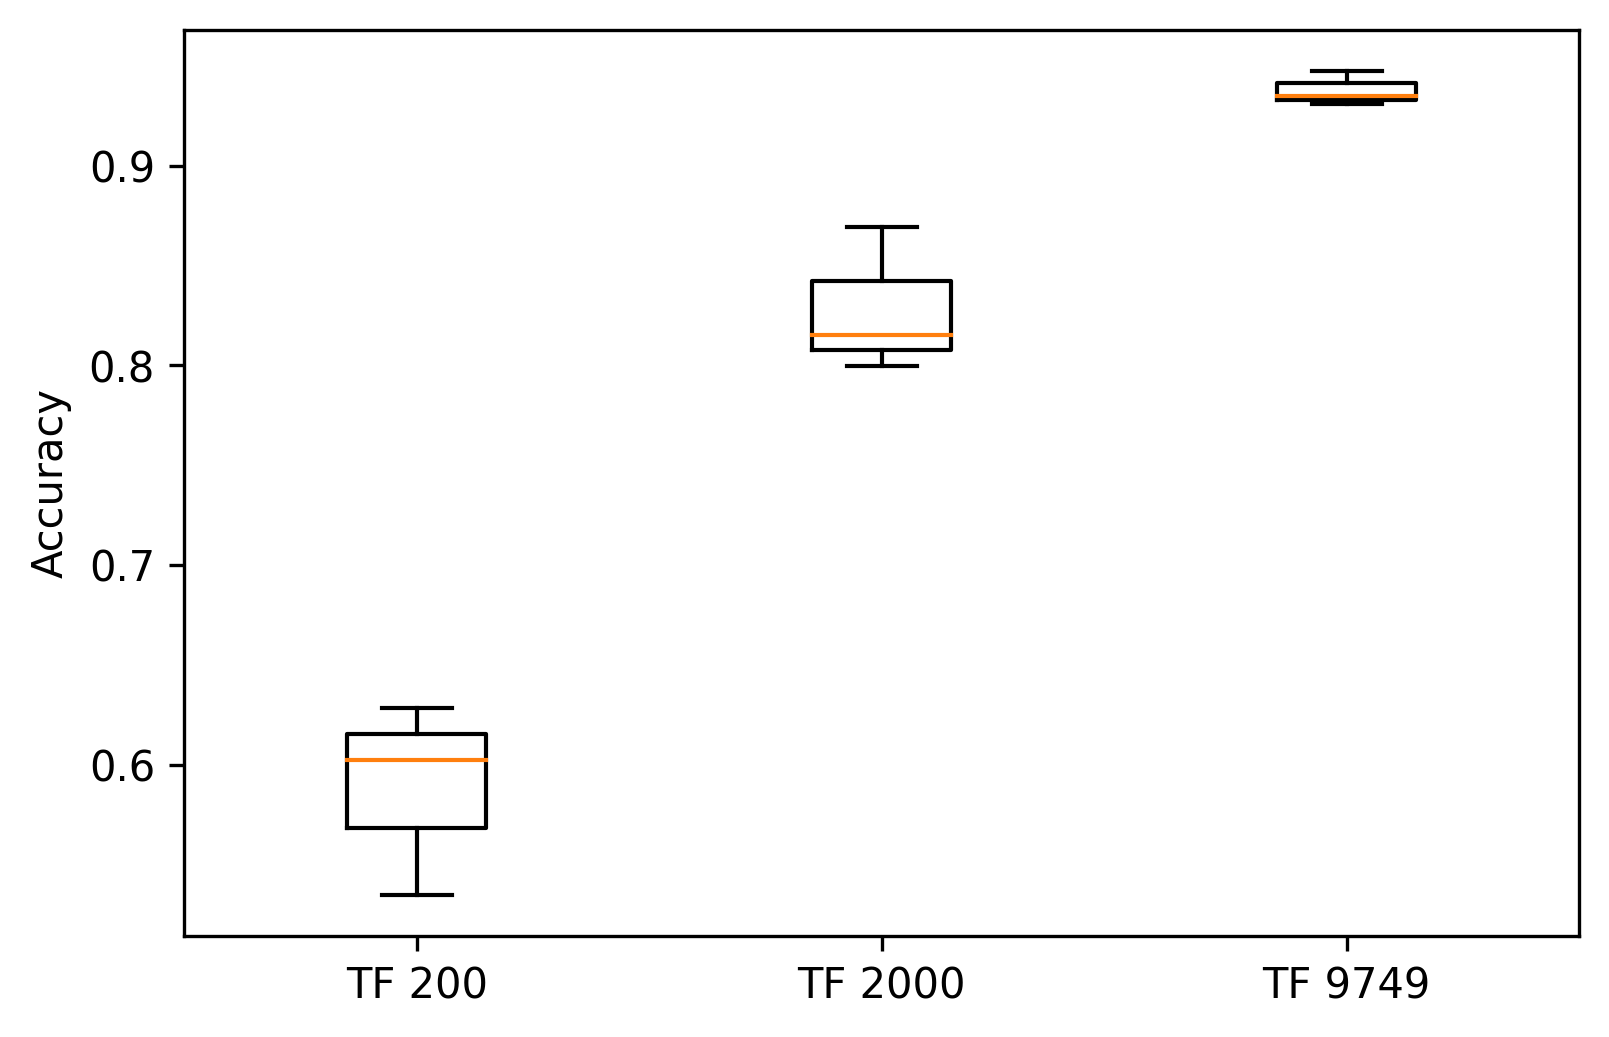
\includegraphics[width=1\textwidth, center]{bilder/Hauptteil/Transfer_Logs_Datenmenge/Acc_MT_Logs_data.png}
			\caption{TFAE Accuracy Datenmenge}
			\label{img:TF_ACC_DATA}	
		\end{subfigure}
	
		\caption{Datenmengen Leistung}
		\label{img:DatenmengenLeistung}
	\end{figure}
		
		
		
		
		
		
		
		
			
		
		
		
		
		
		
		
	
	